%Version 3.1 December 2024
%% Benchmarking multi-paradigma para avaliação integrada da qualidade do solo
%% Manuscrito PT-BR (versão de trabalho) — tradução EN ao final
%%
%%%%%%%%%%%%%%%%%%%%%%%%%%%%%%%%%%%%%%%%%%%%%%%%%%%%%%%%%%%%%%%%%%%%%%

\documentclass[pdflatex,sn-basic]{sn-jnl}% Basic Springer Nature Reference Style

%%%% Standard Packages
\usepackage{graphicx}%
\usepackage{multirow}%
\usepackage{amsmath,amssymb,amsfonts}%
\usepackage{amsthm}%
\usepackage{mathrsfs}%
\usepackage[title]{appendix}%
\usepackage{xcolor}%
\usepackage{textcomp}%
\usepackage{manyfoot}%
\usepackage{booktabs}%
\usepackage{algorithm}%
\usepackage{algorithmicx}%
\usepackage{algpseudocode}%
\usepackage{listings}%
\usepackage{tikz}%
\usetikzlibrary{shapes.geometric, arrows.meta, positioning, calc}%
\usepackage{subcaption}%
\raggedbottom

\begin{document}

\title[Incerteza analítica e risco estocástico]{Incerteza analítica do paradigma estatístico como vetor de risco estocástico na avaliação da qualidade do solo sob manejo conservacionista de longa duração}

%%=============================================================%%
%% Autores
%%=============================================================%%

\author[1]{\fnm{Alceu} \sur{Pedrotti}}\email{alceupedrotti@gmail.com}

\author*[2]{\fnm{Luiz Diego Vidal} \sur{Santos}}\email{ldvsantos@uefs.br}

\author[1]{\fnm{Jusimara de Andrade} \sur{Santos}}\email{jusimara.ufs@gmail.com}

\author[4]{\fnm{Jaelson Souza} \sur{Araújo}}\email{jaelsonagro1207@gmail.com}

\author[1]{\fnm{Sara Julliane de Araújo} \sur{Santos}}\email{sara.julliane@academico.ufs.br}

\author[4]{\fnm{Emersson Guedes da} \sur{Silva}}\email{academicoguedes@gmail.com}

\author[3]{\fnm{Renisson Neponuceno de} \sur{Araújo Filho}}\email{renisson.neponuceno@ufrpe.br}

\author[1]{\fnm{Brisa Marina da Silva} \sur{Andrade}}\email{brisamarina.andrade@gmail.com}

\author[4]{\fnm{Francisco Sandro Rodrigues} \sur{Holanda}}\email{fsrholanda@academico.ufs.br}

\affil[1]{\orgdiv{PRODEMA}, \orgname{Universidade Federal de Sergipe}, \orgaddress{\city{São Cristóvão}, \state{Sergipe}, \country{Brasil}}}

\affil*[2]{\orgdiv{DCHF}, \orgname{Universidade Estadual de Feira de Santana}, \orgaddress{\city{Feira de Santana}, \state{Bahia}, \country{Brasil}}}

\affil[3]{\orgdiv{DTR}, \orgname{Universidade Federal Rural de Pernambuco}, \orgaddress{\city{Recife}, \state{Pernambuco}, \country{Brasil}}}

\affil[4]{\orgdiv{DEA}, \orgname{Universidade Federal de Sergipe}, \orgaddress{\city{São Cristóvão}, \state{Sergipe}, \country{Brasil}}}
%%==================================%%
%% Resumo
%%==================================%%

\abstract{Índices de qualidade do solo (IQS) são amplamente empregados para avaliar manejos conservacionistas, porém a sensibilidade do ranqueamento à escolha do método de agregação permanece pouco quantificada quando famílias estatísticas estruturalmente distintas são confrontadas sobre a mesma base de dados. Neste estudo, comparamos cinco paradigmas (ANOVA/GLM, inferência fuzzy, PLS-SEM, MARS e Random Forest) aplicados a um Argissolo dos Tabuleiros Costeiros monitorado por 22 anos em fatorial de três sistemas de preparo e quatro plantas de cobertura ($n = 108$, 34 indicadores distribuídos em cinco domínios: físico, químico, agronômico, microbiológico e de rendimento). A concordância global foi significativa (Kendall $W = 0{,}73$, $p < 10^{-33}$), porém os paradigmas não lineares (fuzzy, MARS, RF) formaram um bloco praticamente intercambiável ($\rho > 0{,}99$; limites de Bland--Altman $< \pm 0{,}40$), ao passo que ANOVA e PLS-SEM divergiram do bloco não linear ($\bar{\rho}_{\text{Lin-NL}} = 0{,}50$; limites de concordância $\approx \pm 1{,}80$--$2{,}40$), com 67\% das combinações intermediárias de manejo trocando de posição conforme o paradigma. A divergência entre famílias foi confirmada pelo teste de Wilcoxon ($W = 18$, $p = 0{,}012$), indicando que métodos não lineares exibem concordância mútua superior à concordância com paradigmas lineares. Cultivo mínimo com \textit{Cajanus cajan} ocupou a primeira posição em todos os paradigmas, sugerindo que a adoção de pelo menos um método não linear pode reduzir o risco de recomendações conservacionistas dependentes do algoritmo.}

\keywords{índice de qualidade do solo, sistema de inferência fuzzy, PLS-SEM, MARS, Random Forest, ANOVA, comparação metodológica, fertilidade química, microbiologia do solo, plantas de cobertura, sistemas de manejo}

\maketitle

%% ================================================================
%%                    SEÇÃO 1: INTRODUÇÃO
%% ================================================================
\section{Introdução}\label{sec:intro}

A degradação do solo compromete a capacidade produtiva de aproximadamente 33\% das terras agrícolas globais, com perdas anuais estimadas entre 25 e 40 bilhões de toneladas de solo fértil por erosão hídrica \citep{Lal2015}. Nos trópicos úmidos, onde a mineralização acelerada da matéria orgânica e a agressividade das chuvas intensificam esses processos, a adoção de sistemas conservacionistas (plantio direto, cultivo mínimo e uso de plantas de cobertura) tornou-se estratégia central para a manutenção das funções edáficas \citep{Doran2002,Cardoso2013}. A avaliação quantitativa da eficácia dessas práticas requer ferramentas que integrem atributos físicos, químicos e biológicos em métricas auditáveis, o que motivou o desenvolvimento dos índices de qualidade do solo (IQS) \citep{Karlen1997}.

O conceito de IQS consolidou-se a partir do arcabouço proposto por \cite{Karlen1997} e do protocolo operacional de \cite{Andrews2002}, que estabeleceu a seleção de conjunto mínimo de dados (MDS) por análise de componentes principais (ACP) seguida de escorificação aditiva. Desde então, revisões abrangentes documentaram a proliferação de variantes metodológicas, com mais de 60 combinações de seleção, ponderação e agregação publicadas até 2018 \citep{Bünemann2018}. Essa diversidade, embora sinal de maturidade da área, introduz um problema de comparabilidade entre estudos que adotam paradigmas distintos para os mesmos indicadores.

Na abordagem clássica, modelos paramétricos (ANOVA ou GLM) produzem escores lineares a partir de pesos derivados de autovalores da ACP, supondo que as relações entre indicadores e qualidade do solo são monotônicas e aditivas \citep{Mukherjee2014}. A simplicidade computacional e a transparência interpretativa tornaram esse paradigma predominante em avaliações de manejo conservacionista, inclusive em experimentos de longa duração sobre Argissolos dos Tabuleiros Costeiros do Nordeste brasileiro \citep{Assuncao2023}. A limitação reside na incapacidade do modelo linear de capturar efeitos limiares e interações de ordem superior entre indicadores de domínios distintos \citep{DosSantos2021}.

Sistemas de inferência fuzzy (SIF) foram introduzidos como alternativa para acomodar a incerteza de fronteira inerente à classificação de indicadores contínuos em categorias discretas de qualidade \citep{Torbert2008}. Ao substituir cortes rígidos por funções de pertinência triangulares ou gaussianas, o SIF preserva a gradação dos atributos edáficos e permite a incorporação de conhecimento especializado por meio de bases de regras linguísticas \citep{Nabiollahi2018}. Aplicações recentes em solos tropicais brasileiros indicaram que o SIF pode detectar diferenças de manejo que o protocolo aditivo clássico não distingue \citep{DosSantos2021}, embora a calibração das funções de pertinência permaneça dependente de dados regionais nem sempre disponíveis.

Algoritmos de aprendizado de máquina (AM), a exemplo de \textit{Random Forest} (RF) e \textit{Multivariate Adaptive Regression Splines} (MARS), exploram não linearidade e interação de alta ordem por meio de particionamento recursivo do espaço de preditores \citep{Zeraatpisheh2020}. O RF, em particular, oferece métricas intrínsecas de importância de variáveis (por permutação ou impureza) e estimativas \textit{out-of-bag} que dispensam validação cruzada explícita, o que o tornou popular em mapeamento digital de solos \citep{Wadoux2020}. O MARS, por sua vez, identifica limiares (\textit{knots}) adaptativos que aproximam descontinuidades na resposta sem recorrer à discretização prévia dos indicadores. A interpretabilidade do AM, porém, é inferior à dos modelos estatísticos clássicos, e o risco de sobreajuste em amostras pequenas ($n < 50$) requer atenção \citep{Chaudhry2024}.

A modelagem de equações estruturais por mínimos quadrados parciais (PLS-SEM) ocupa posição intermediária entre os paradigmas anteriores. Ao especificar construtos latentes que representam domínios edáficos (físico, agronômico, rendimento) e estimar coeficientes de caminho entre eles, o PLS-SEM testa hipóteses causais sobre a cadeia solo--planta--rendimento \citep{Hair2019,Sarstedt2022}. A especificação mista (Mode~A reflexivo para indicadores que manifestam o construto e Mode~B formativo para indicadores que causam o construto) confere flexibilidade teórica \citep{Diamantopoulos2008}, embora a linearidade dos caminhos estruturais limite a captura de interações não lineares entre domínios.

Na prática, cada estudo ambiental opta por um único paradigma algorítmico e assume, implicitamente, que a classificação das combinações de manejo é determinística e estável frente à escolha metodológica. Entretanto, a literatura recente sobre modelagem ambiental indica que ignorar não linearidades intrínsecas aos ecossistemas terrestres introduz incerteza analítica que se propaga para as decisões de manejo \citep{Yoshioka2024,Brito2024}. Quando restrita a modelos de compressão linear, a predição da qualidade do solo omite dinâmicas de limiar e interações de alta ordem, elevando o risco de falsos positivos na recomendação de práticas agrícolas em domínios ambientais complexos. Algoritmos de aprendizado de máquina adaptativos, como \textit{Random Forest}, tendem a reduzir essa incerteza preditiva, uma vez que modelos \textit{ensemble} lidam mais adequadamente com o ruído probabilístico da amostragem em campo \citep{Granata2024}.

Comparações recentes envolvendo variantes de escorificação \citep{Mukherjee2014}, aprendizado de máquina \citep{Chaudhry2024} e lógica fuzzy--AHP \citep{Pacci2026} abordaram marginalmente o problema para IQS, porém restringiram-se a subconjuntos da mesma família analítica e não empregaram métricas formais de concordância inter-avaliador \citep{Venkateswarlu2025,Liu2025}. Em contextos de suporte à decisão sob incerteza, a ausência de protocolos de concordância entre famílias estatísticas pode propagar viés algorítmico para recomendações de manejo, comprometendo a confiabilidade do processo decisório em escalas de paisagem \citep{Angelini2024,Jarvis2023}. Faltam, portanto, evidências empíricas que quantifiquem o risco de alteração do ranqueamento de manejos quando paradigmas estruturalmente distintos (lineares e não lineares) são aplicados simultaneamente sobre o mesmo conjunto de dados edáficos.

Os Argissolos dos Tabuleiros Costeiros do Nordeste brasileiro, derivados de sedimentos da Formação Barreiras, apresentam horizonte A franco-arenoso e camada coesa em subsuperfície que limita a drenagem interna e a penetração radicular \citep{LimaNeto2010}. Nessas condições, os sistemas conservacionistas melhoram indicadores físicos e biológicos por meio de gradientes contínuos e frequentemente sutis \citep{Assuncao2023,Oliveira2020}. Se os métodos estatísticos divergem justamente nas faixas limites desses gradientes, a utilidade prática do IQS pode ser comprometida, tornando as recomendações de manejo dependentes do algoritmo empregado \citep{Rezaee2020,Obade2016}.

Este estudo avalia a incerteza analítica em índices de qualidade do solo (IQS) imposta pela escolha do método de agregação e quantifica o risco de alteração do ranqueamento de manejos conservacionistas. Para tanto, comparamos cinco abordagens analíticas de famílias estruturalmente distintas (ANOVA/GLM, SIF, PLS-SEM, MARS e RF) aplicadas ao mesmo conjunto de dados ($n = 108$, 34 indicadores distribuídos em cinco domínios, três sistemas de manejo e quatro espécies de cobertura em experimento de 22 anos). O vetor de indicadores reúne atributos físicos, químicos, microbiológicos, agronômicos e de rendimento obtidos em duas campanhas amostrais complementares na mesma área experimental, conferindo representatividade aos domínios exigidos em protocolos internacionais de qualidade do solo \citep{Karlen1997,Andrews2002}.

Se os cinco paradigmas acessam estruturas de variância compatíveis, espera-se que a concordância de ranqueamento seja estatisticamente diferente de zero ($W > 0$, $\alpha = 0{,}05$). Essa convergência, contudo, pode não ser homogênea entre famílias analíticas, de modo que métodos não lineares (SIF, MARS, RF) tenderiam a exibir maior concordância mútua do que com paradigmas lineares. Adicionalmente, a estabilidade da concordância pode depender do tamanho amostral, crescendo log-linearmente até estabilizar a partir de um limiar amostral crítico.

%% ================================================================
%%                    SEÇÃO 2: MATERIAL E MÉTODOS
%% ================================================================
\section{Material e Métodos}\label{sec:material}

\subsection{Descrição do conjunto de dados}\label{subsec:dataset}

O conjunto de dados utilizado neste \textit{benchmarking} foi obtido em experimento de campo de longa duração conduzido na Estação Experimental da Universidade Federal de Sergipe, município de São Cristóvão, SE (10$^\circ$55$'$24$''$\,S, 37$^\circ$11$'$57$''$\,W, 22\,m de altitude), conforme ilustrado na Fig.~\ref{fig:site}. O clima regional é classificado como As$'$ (tropical chuvoso com verão seco) segundo Köppen, com precipitação anual de aproximadamente 1\,600\,mm concentrada entre abril e setembro. O solo é um Argissolo Vermelho Amarelo Distrófico (\textit{Acrisol}, WRB; \textit{Typic Hapludult}, USDA), derivado da Formação Barreiras, com horizonte A franco-arenoso e presença de camada coesa em subsuperfície. O experimento foi instalado em 2001 em delineamento de faixas subdivididas (\textit{strip-split plot}) com subparcelas de 6\,m\,$\times$\,10\,m, e os dados analisados correspondem ao 22$^\circ$ ano de condução contínua (safra 2022). A avaliação do IQS pelo método aditivo clássico, referente ao 17$^\circ$ ano desse experimento, foi publicada por \cite{Assuncao2023}; o presente estudo amplia essa base ao aplicar cinco paradigmas analíticos à safra 2022.

\begin{figure}[ht]
\centering
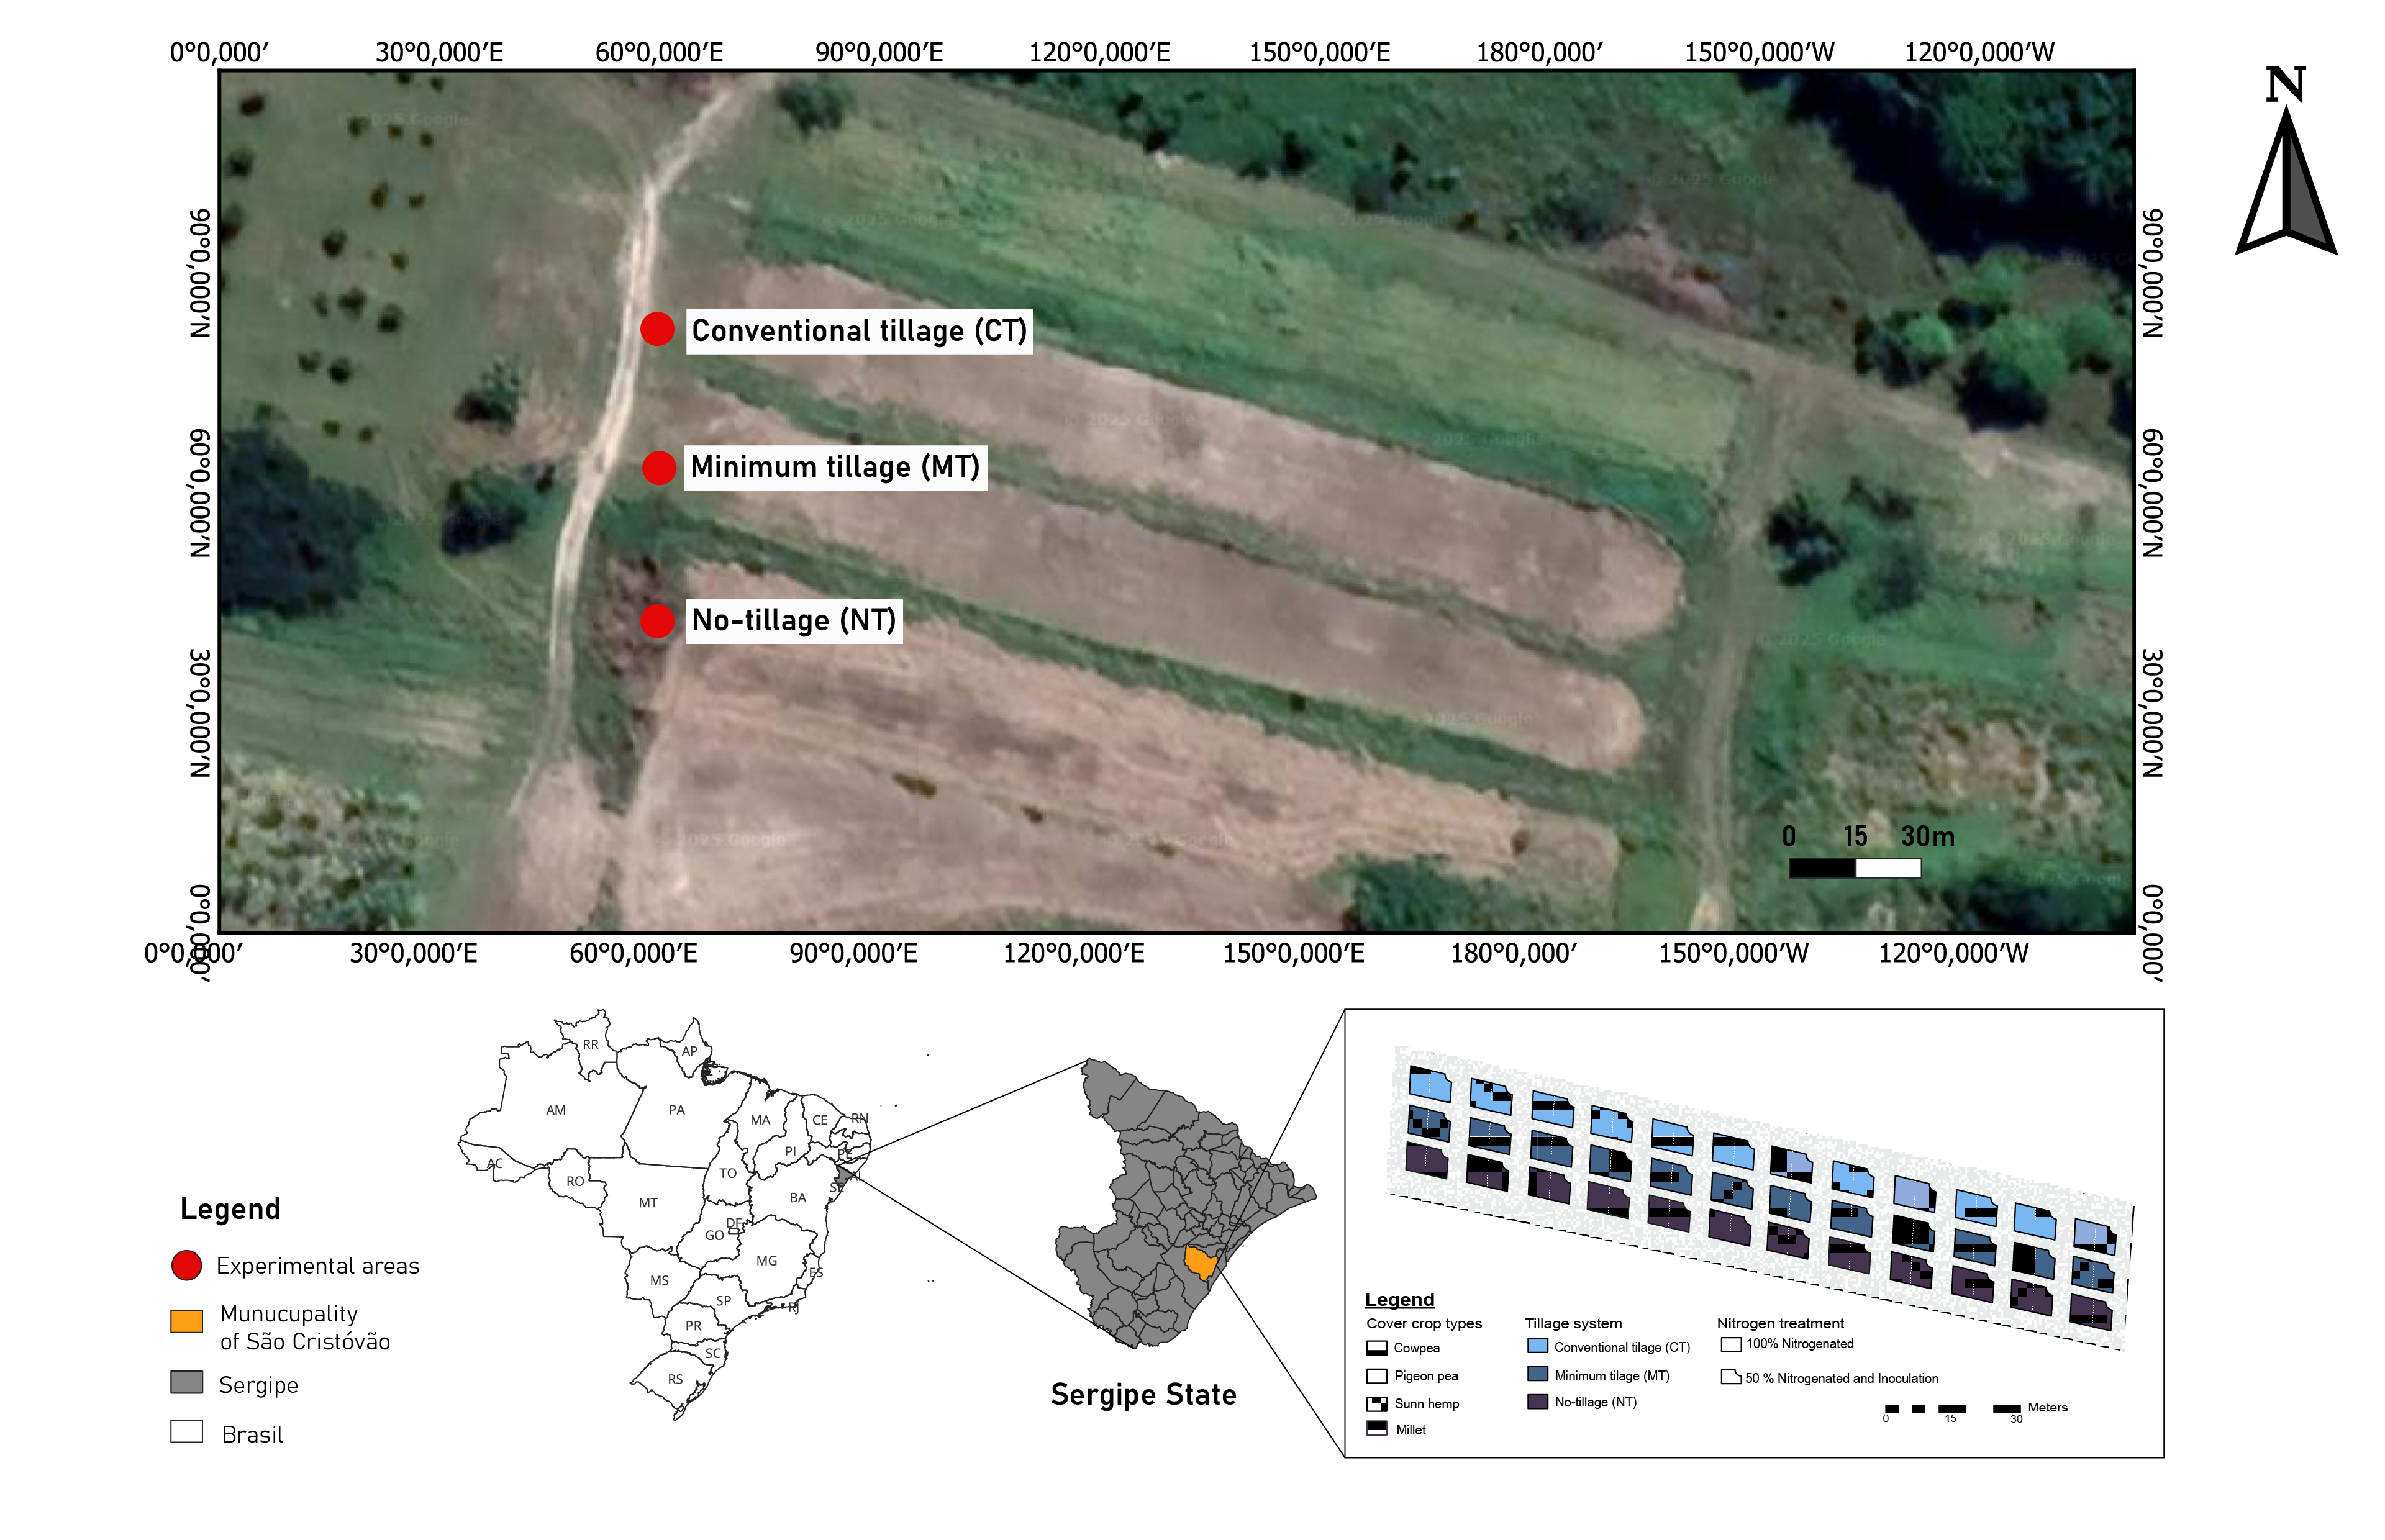
\includegraphics[width=0.85\textwidth]{../../2-DADOS/3-FIGURAS/fig_experimental_site.jpg}
\caption{Localização e vista geral do experimento de longa duração (implantado em 2001) na Estação Experimental da Universidade Federal de Sergipe, município de São Cristóvão, SE, sobre Argissolo Vermelho Amarelo Distrófico dos Tabuleiros Costeiros.}\label{fig:site}
\end{figure}

As observações ($n = 108$) foram coletadas em delineamento fatorial que combinou três sistemas de manejo do solo (plantio direto, PD; plantio convencional, PC; e cultivo mínimo, CM) com quatro espécies de plantas de cobertura (feijão-caupi, \textit{Vigna unguiculata}; milheto, \textit{Pennisetum glaucum}; feijão-guandu, \textit{Cajanus cajan}; e crotalária, \textit{Crotalaria juncea}), totalizando 12 combinações com nove repetições cada. A cultura principal \textit{Zea mays} L. (híbrido SHS7990 PRO3) foi semeada no espaçamento de 0,80\,m\,$\times$\,0,20\,m ($\approx$\,54\,000\,plantas\,ha$^{-1}$), precedida pela cobertura semeada manualmente 90 dias antes. O plantio convencional consistiu em aração com disco a 25\,cm seguida de grade niveladora, o cultivo mínimo empregou apenas grade niveladora e o plantio direto dispensou revolvimento mecânico.

Com nove repetições por célula fatorial ($3 \times 4 = 12$ combinações), o delineamento totaliza $n = 108$ observações. A análise de poder \textit{a posteriori} para a ANOVA fatorial com $\alpha = 0{,}05$, tamanho de efeito médio ($f = 0{,}25$) e $k = 12$ grupos indica poder estatístico $> 0{,}90$ para detectar diferenças entre combinações de manejo, atendendo ao limiar recomendado por \cite{Mundform2005} para análises multivariadas.

A amostragem restringiu-se à camada 0--0,20~m por razões operacionais, uma vez que a camada coesa neste Argissolo situa-se entre 0,25 e 0,45~m de profundidade \citep{LimaNeto2010} e a coleta em profundidades inferiores exigiria trincheiras em todas as 108 parcelas, inviável no contexto de experimento de longa duração com parcelas de 60~m$^2$. Essa restrição pode subestimar a diferenciação física entre tratamentos que atuam sobre a camada coesa (e.g., raiz pivotante do guandu), constituindo limitação reconhecida deste estudo.

\subsection{Indicadores de solo e planta}\label{subsec:indicators}

Trinta e quatro indicadores distribuídos em cinco domínios (físico do solo, químico, microbiológico, agronômico e de rendimento) foram mensurados (Tabela~\ref{tab:indicators}). Os indicadores físicos (DMG, DMP, Ds, RMP, Na, COS, ICV, MI, MA, VIB, RP, AD/PT), agronômicos (ALT, DESP, CESP, STAND) e de rendimento (NESP, NESPC, PESP, PROD) foram obtidos na safra 2022 do presente experimento. Os indicadores químicos (pH, P, K, Ca, Mg, Al, CTC, MOS, EstN) e microbiológicos (qMIC, qCO2, CCO2, CMIC, NMIC) foram obtidos em avaliação complementar conduzida nas mesmas parcelas experimentais por \cite{Sara2019}, na profundidade de 0--10\,cm, e integrados ao conjunto de dados como médias por célula do delineamento (manejo\,$\times$\,cobertura). A integração de duas campanhas amostrais na mesma área experimental é justificada pela estabilidade temporal dos atributos edáficos em experimentos de longa duração ($> 15$ anos) conduzidos sobre Argissolos dos Tabuleiros Costeiros \citep{Assuncao2023}, nos quais a diferenciação entre tratamentos resulta de efeitos cumulativos que se sobrepõem à variabilidade interanual.

O pH foi determinado em suspensão solo:água (1:2,5) com potenciômetro calibrado (precisão $\pm 0{,}02$), o P e K disponíveis por Mehlich-1 com leitura em espectrofotômetro UV-Vis a 725\,nm e fotômetro de chama, respectivamente (CV analítico $< 5$\%). O Ca e Mg trocáveis foram extraídos com KCl 1\,mol\,L$^{-1}$ e determinados por espectrofotometria de absorção atômica. O Al trocável foi extraído com KCl 1\,mol\,L$^{-1}$ e titulado com NaOH 0,025\,mol\,L$^{-1}$. A CTC a pH~7 foi calculada pela soma de bases e acidez potencial. A matéria orgânica do solo (MOS) foi determinada pelo método Walkley-Black modificado (CV $< 6$\%) e o estoque de nitrogênio (EstN) por digestão Kjeldahl. O estoque de carbono orgânico do solo (COS) foi determinado pelo método Walkley-Black.

Os indicadores microbiológicos (CMIC e NMIC) foram determinados pelo método fumigação-extração \citep{Vance1987}, a respiração basal do solo (CCO2) por captura de CO$_2$ em NaOH, e os quocientes metabólico (qCO2) e microbiano (qMIC) foram calculados como razões derivadas. A microporosidade (MI) e macroporosidade (MA) foram obtidas por mesa de tensão, a velocidade de infiltração básica (VIB) por infiltrômetro de anel duplo, a resistência à penetração (RP) por penetrômetro de impacto e a razão água disponível/porosidade total (AD/PT) foi calculada a partir da curva de retenção.

A inclusão dos 16 indicadores adicionais (9 químicos e 5 microbiológicos da campanha complementar, mais 5 físicos) demandou recalibração das funções de pertinência do SIF (ampliação do universo de discurso), reajuste dos hiperparâmetros de RF (\texttt{mtry} recalculado para $\lfloor \sqrt{34} \rfloor = 6$) e MARS (reprocessamento de \textit{forward/backward}), além de re-especificação do modelo PLS-SEM com cinco construtos (inclusão do construto MICROBIOLÓGICO), de modo que todos os paradigmas foram re-estimados com o vetor completo de 34 indicadores. A razão $n/p = 108/34 \approx 3{,}2$ situa-se abaixo do limiar $n/p = 5$ recomendado para PLS-SEM \citep{Hair2019}, condição que foi mitigada pela triagem de multicolinearidade (VIF\,$> 5$) que reduziu o modelo estrutural a 25 indicadores.

\begin{table}[h]
\caption{Indicadores de solo e planta utilizados na análise de \textit{benchmarking}.}\label{tab:indicators}
\begin{tabular*}{\textwidth}{@{\extracolsep\fill}llll}
\toprule
Domínio & Indicador & Sigla & Unidade \\
\midrule
\multirow{12}{*}{Físico do solo} 
  & Diâmetro médio geométrico & DMG & mm \\
  & Diâmetro médio ponderado & DMP & mm \\
  & Densidade do solo & Ds & Mg\,m$^{-3}$ \\
  & Persistência de umidade residual & RMP & -- \\
  & Agregados estáveis em água & Na & \% \\
  & Estoque de carbono orgânico do solo & COS & Mg\,ha$^{-1}$ \\
  & Índice de cobertura vegetal & ICV & \% \\
  & Microporosidade & MI & m$^3$\,m$^{-3}$ \\
  & Macroporosidade & MA & m$^3$\,m$^{-3}$ \\
  & Velocidade de infiltração básica & VIB & cm\,h$^{-1}$ \\
  & Resistência à penetração & RP & MPa \\
  & Água disponível / porosidade total & AD/PT & -- \\
\midrule
\multirow{9}{*}{Químico do solo}
  & pH em água (0--10\,cm) & pH & -- \\
  & Fósforo disponível (0--10\,cm) & P & mg\,dm$^{-3}$ \\
  & Potássio disponível (0--10\,cm) & K & mg\,dm$^{-3}$ \\
  & Cálcio trocável & Ca & cmol$_c$\,dm$^{-3}$ \\
  & Magnésio trocável & Mg & cmol$_c$\,dm$^{-3}$ \\
  & Alumínio trocável & Al & cmol$_c$\,dm$^{-3}$ \\
  & Capacidade de troca catiônica & CTC & cmol$_c$\,dm$^{-3}$ \\
  & Matéria orgânica do solo & MOS & g\,kg$^{-1}$ \\
  & Estoque de nitrogênio & EstN & Mg\,ha$^{-1}$ \\
\midrule
\multirow{5}{*}{Microbiológico}
  & Carbono da biomassa microbiana & CMIC & mg\,C\,kg$^{-1}$ \\
  & Nitrogênio da biomassa microbiana & NMIC & mg\,N\,kg$^{-1}$ \\
  & Respiração basal do solo & CCO2 & mg\,C-CO$_2$\,kg$^{-1}$\,dia$^{-1}$ \\
  & Quociente metabólico & qCO2 & mg\,C-CO$_2$\,mg$^{-1}$\,CMIC\,dia$^{-1}$ \\
  & Quociente microbiano & qMIC & \% \\
\midrule
\multirow{4}{*}{Agronômico} 
  & Altura de plantas & ALT & cm \\
  & Diâmetro da espiga & DESP & mm \\
  & Comprimento da espiga & CESP & cm \\
  & Estande final & STAND & plantas\,ha$^{-1}$ \\
\midrule
\multirow{4}{*}{Rendimento} 
  & Número total de espigas por hectare & NESP & espigas\,ha$^{-1}$ \\
  & Espigas comerciais por hectare & NESPC & espigas\,ha$^{-1}$ \\
  & Peso de espigas comerciais por hectare & PESP & kg\,ha$^{-1}$ \\
  & Produtividade & PROD & kg\,ha$^{-1}$ \\
\botrule
\end{tabular*}
\smallskip\noindent\textit{Nota:} Todos os indicadores foram normalizados para a escala 0--10 previamente à aplicação dos paradigmas fuzzy e de AM. Indicadores químicos e microbiológicos foram obtidos em avaliação complementar \citep{Sara2019} na mesma área experimental e integrados como médias por célula do delineamento. Indicadores físicos MI, MA, VIB, RP e AD/PT também provêm da campanha complementar.
\end{table}

\subsection{Paradigma 1: ANOVA/GLM com seleção de conjunto mínimo de dados}\label{subsec:anova}

A abordagem clássica foi incluída por representar o paradigma mais difundido na literatura de IQS e por operar sob pressupostos de aditividade e monotonicidade que servem de linha-base para aferir o ganho informacional dos métodos não lineares. O mecanismo de captura da variabilidade restringe-se à decomposição linear de variância por autovalores de ACP, o que implica que interações de ordem superior e efeitos limiares entre domínios edáficos permaneçam no resíduo não explicado.

Modelos lineares generalizados (GLM) foram ajustados para cada indicador conforme o protocolo de \cite{Andrews2002}, segundo
\begin{equation}
Y_{ijk} = \mu + \alpha_i + \beta_j + (\alpha\beta)_{ij} + \varepsilon_{ijk}
\label{eq:glm}
\end{equation}
em que $\alpha_i$ representa o efeito do sistema de manejo ($i = 1, 2, 3$), $\beta_j$ o efeito da espécie de cobertura ($j = 1, \ldots, 4$), $(\alpha\beta)_{ij}$ a interação entre ambos e $\varepsilon_{ijk}$ o erro residual. A ANOVA tipo~II foi processada com o pacote \texttt{car}. Comparações múltiplas entre médias foram realizadas por médias marginais estimadas (\texttt{emmeans}) com ajuste de Tukey.

A seleção de conjunto mínimo de dados (MDS) foi conduzida via ACP. Indicadores com cargas fatoriais superiores a 0,70 em cada componente retido foram identificados e, dentre indicadores correlacionados dentro de cada componente, aquele com maior comunalidade foi retido. O IQS linear foi computado como
\begin{equation}
\text{IQS}_{\text{ANOVA}} = \sum_{i=1}^{k} w_i \cdot S_i
\label{eq:sqi_anova}
\end{equation}
em que $w_i$ corresponde ao peso derivado dos autovalores da ACP e $S_i$ ao escore normalizado de cada indicador. A normalidade dos resíduos do GLM foi avaliada pelo teste de Shapiro-Wilk e a homocedasticidade pelo teste de Levene (pacote \texttt{car}). Indicadores cujos resíduos violaram o pressuposto de normalidade ($p < 0{,}05$) foram transformados por Box-Cox previamente à ANOVA; quando a transformação não normalizou os resíduos, empregou-se ANOVA não paramétrica (Kruskal-Wallis) seguida de teste de Dunn com ajuste de Bonferroni.

\subsection{Paradigma 2: Sistema de inferência fuzzy}\label{subsec:fuzzy}

A inferência fuzzy foi selecionada por sua capacidade de acomodar a transição gradual entre classes de qualidade edáfica sem impor fronteiras rígidas sobre indicadores contínuos. O mecanismo opera pela sobreposição de funções de pertinência que atribuem graus parciais de associação a cada categoria linguística, preservando a incerteza inerente à fronteira entre "baixo" e "médio" ou "médio" e "alto" que a escorificação aditiva elimina ao discretizar indicadores em escores 0--1. Dessa forma, efeitos de limiar que a combinação linear comprime podem ser captados pela base de regras sem necessidade de especificação paramétrica prévia.

Um sistema de inferência fuzzy do tipo Mamdani \citep{Mamdani1975} foi construído segundo o arcabouço de \cite{Torbert2008}. Cada um dos 15 indicadores originais foi fuzzificado em três categorias linguísticas (baixo, médio, alto) com funções de pertinência triangulares e, separadamente, gaussianas. As funções triangulares foram definidas como
\begin{equation}
\mu_A(x) = \max\left(\min\left(\frac{x-a}{b-a},\; \frac{c-x}{c-b}\right),\; 0\right)
\label{eq:trimf}
\end{equation}
em que $a$, $b$ e $c$ delimitam o suporte e o pico do conjunto fuzzy. As funções gaussianas seguiram
\begin{equation}
\mu_A(x) = \exp\left(-\frac{(x-c)^2}{2\sigma^2}\right)
\label{eq:gaussmf}
\end{equation}

A base de regras foi elaborada a partir de conhecimento especializado e a defuzzificação realizada pelo método do centróide. A saída, denominada Índice de Performance e Conservação do Solo Integrado (IPACSA), foi computada na escala 0--10 com o pacote \texttt{FuzzyR}.

\subsection{Paradigma 3: Modelagem de equações estruturais PLS-SEM}\label{subsec:sem}

O PLS-SEM foi incluído por possibilitar a especificação de relações direcionais entre domínios edáficos (físico, químico, microbiológico, agronômico, rendimento) como construtos latentes, testando hipóteses causais explícitas sobre a cadeia solo--planta--rendimento. O mecanismo de captura reside na estimação de coeficientes de caminho que ponderam a contribuição relativa de cada domínio para o rendimento, enquanto a especificação formativa (Mode~B) permite que indicadores como pH, P, Ca e CMIC atuem como determinantes da fertilidade e da atividade biológica e não como manifestações reflexivas de um fator latente. Essa flexibilidade distingue o PLS-SEM dos demais paradigmas ao incorporar uma estrutura teórica na agregação, embora a linearidade dos caminhos estruturais limite a captura de interações de ordem superior.

Um modelo de caminhos PLS hierárquico foi especificado com cinco construtos latentes de primeira ordem (FÍSICO, QUÍMICO, MICROBIOLÓGICO, AGRONÔMICO e RENDIMENTO) e um construto de segunda ordem, IQS. O modelo estrutural especificou caminhos direcionais conforme
\begin{equation}
\text{IQS}_{\text{PLS}} = \gamma_1 \cdot \eta_{\text{FIS}} + \gamma_2 \cdot \eta_{\text{QUIM}} + \gamma_3 \cdot \eta_{\text{MICRO}} + \gamma_4 \cdot \eta_{\text{AGRO}} + \gamma_5 \cdot \eta_{\text{REND}} + \zeta
\label{eq:plssem}
\end{equation}
Indicadores como densidade do solo (Ds) e produção de espigas (PESP, NESPC) atuam como causas (e não como reflexos) de seus respectivos construtos, o que implica relações formativas. Por essa razão, o modelo adotou especificação formativa (Mode~B) para todos os construtos. Uma triagem de multicolinearidade (VIF\,$> 5$) excluiu quatro indicadores com inflação excessiva: CTC (VIF\,=\,37,5), EstN (VIF\,=\,13,7), CMIC (VIF\,=\,23,9) e PROD (VIF\,=\,20,1), resultando em 25 indicadores distribuídos entre os cinco construtos de primeira ordem: FÍSICO (Mode~B: DMG, DMP, Ds, RMP, Na, COS, ICV, MI, MA), QUÍMICO (Mode~B: pH, P, K, Ca, Mg, Al, MOS), MICRO (Mode~B: qMIC, qCO2, CCO2, NMIC), AGRO (Mode~B: ALT, DESP, CESP, STAND) e REND (Mode~B: NESP, NESPC, PESP). A validação de Mode~B seguiu critérios de significância dos pesos externos (\textit{outer weights}) e ausência de multicolinearidade residual.

A estimação seguiu abordagem em dois estágios (\textit{two-stage approach}) com o pacote \texttt{seminr} \citep{Ray2022}. A qualidade global do modelo foi avaliada pelo SRMR (\textit{Standardized Root Mean Square Residual}), com limiar de aceitação $< 0{,}08$ \citep{Hair2019}, e pelo \textit{Goodness of Fit} (GoF) como média geométrica entre comunalidades médias e $R^2$ médio dos construtos endógenos. Para os construtos formativos (Mode~B), aplicou-se teste de redundância por correlação entre o escore formativo e um indicador global reflexivo, verificando-se validade convergente quando $r > 0{,}70$. No primeiro estágio, os cinco construtos de primeira ordem (FÍSICO, QUÍMICO, MICRO, AGRO, REND) foram estimados iterativamente, com caminhos estruturais FÍSICO$\to$REND, QUÍMICO$\to$REND, MICRO$\to$REND e AGRO$\to$REND. No segundo estágio, os escores latentes dos cinco construtos foram submetidos a ACP, e o primeiro componente principal foi adotado como IQS$_{\text{PLS}}$, escalado para o intervalo 0--10. Intervalos de confiança dos coeficientes de caminho foram obtidos por \textit{bootstrap} de 500 reamostras.

\subsection{Paradigma 4: MARS com análise de ablação}\label{subsec:mars}

O MARS foi selecionado por identificar descontinuidades na resposta por meio de funções-dobradiça (\textit{hinge functions}) que segmentam o espaço de preditores em regiões lineares locais, sem exigir discretização prévia nem especificação do número ou posição dos limiares. O mecanismo de captura da não linearidade reside na seleção automática de nós adaptativos (\textit{knots}) pelo algoritmo de adição progressiva e poda reversa, que aproximam relações cuja curvatura varia ao longo da faixa de valores dos indicadores.

Modelos MARS \citep{Friedman1991} foram ajustados com o pacote \texttt{earth} \citep{Milborrow2023} para capturar relações não lineares entre indicadores e uma variável-alvo (rendimento ou IQS composto). O modelo selecionou funções-base por adição progressiva (\textit{forward stepwise}) e poda reversa (\textit{backward pruning}) conforme
\begin{equation}
\hat{f}(x) = \beta_0 + \sum_{m=1}^{M} \beta_m \prod_{k=1}^{K_m} h_{km}(x_{v(k,m)})
\label{eq:mars}
\end{equation}
em que $h_{km}$ são funções-dobradiça (\textit{hinge}) da forma $\max(0, x - t)$ ou $\max(0, t - x)$.

A importância das variáveis foi avaliada por análise de ablação, na qual cada indicador foi sequencialmente removido e o deslocamento absoluto médio do ranqueamento (\textit{Mean Absolute Rank Shift}) quantificou o impacto sobre o IQS predito. 

Indicadores cujo escore de ablação superou um limiar pré-definido foram classificados como insubstituíveis para o índice. A adequação dos nós adaptativos foi verificada por diagrama Resíduos $\times$ Valores Ajustados e pelo teste de Breusch-Pagan para heterocedasticidade (pacote \texttt{lmtest}); a ausência de padrão sistemático nos resíduos e $p > 0{,}05$ no teste BP confirmam que as funções-dobradiça capturam adequadamente a estrutura de variância dos dados. Adicionalmente, a importância global das variáveis foi estimada por valores SHAP (\textit{SHapley Additive exPlanations}) com o pacote \texttt{DALEX}, possibilitando comparação direta com as métricas de importância do RF e alinhamento interpretativo entre paradigmas.

\subsection{Paradigma 5: Regressão por \textit{Random Forest}}\label{subsec:rf}

O RF \citep{Breiman2001} foi incluído por sua capacidade de capturar interações de alta ordem e não linearidades por meio de particionamento recursivo do espaço de preditores em um \textit{ensemble} de árvores de decisão independentes. O mecanismo opera pela agregação \textit{bootstrap} (\textit{bagging}) de múltiplas árvores treinadas em subconjuntos aleatórios de observações e variáveis, o que reduz a variância das predições e fornece estimativas internas de erro (OOB) que dispensam partição explícita treino/teste.

Modelos de \textit{Random Forest} foram treinados com o pacote \texttt{randomForest} utilizando 500 árvores, $\lfloor \sqrt{q} \rfloor = 6$ variáveis amostradas aleatoriamente em cada divisão e tamanho mínimo de nó terminal igual a~5. A escolha de $\text{mtry} = \lfloor \sqrt{q} \rfloor$ em vez de $\lfloor q/3 \rfloor$ reduz a correlação entre árvores e confere maior estabilidade ao \textit{ensemble} quando a razão $n/q$ é moderada ($\approx 3{,}2$), condição presente nesta base de dados. A convergência do erro \textit{out-of-bag} (OOB-MSE) foi verificada por meio de curva OOB-MSE $\times$ número de árvores, e estimativas de erro OOB forneceram métrica interna de validação. A importância das variáveis foi quantificada por duas vias complementares, o incremento percentual no erro quadrático médio (\%IncMSE) após permutação de cada preditor e valores SHAP globais obtidos com o pacote \texttt{DALEX} (500 permutações). 

Intervalos de confiança a 95\% para as predições de IQS foram estimados pelo método \textit{infinitesimal jackknife} \citep{Wager2014} implementado no pacote \texttt{randomForestCI}. Além do $R^2_{\text{OOB}}$, reportou-se o OOB-RMSE em unidades originais da escala 0--10 para permitir interpretação direta da magnitude do erro preditivo. O IQS predito foi definido como
\begin{equation}
\text{IQS}_{\text{RF}} = \frac{1}{B}\sum_{b=1}^{B} T_b(\mathbf{x})
\label{eq:rf}
\end{equation}
em que $T_b$ corresponde à predição da árvore $b$ para a observação $\mathbf{x}$.

\subsection{Avaliação da concordância inter-paradigma}\label{subsec:concordance}

Os cinco paradigmas geram valores de IQS em escalas distintas. Previamente à comparação, todos os vetores de IQS foram padronizados pela transformação normal inversa baseada em postos \citep{Blom1958}, conforme
\begin{equation}
z_i = \Phi^{-1}\!\left(\frac{r_i - 0{,}5}{n}\right)
\label{eq:blom}
\end{equation}
em que $r_i$ é o posto da observação $i$ e $\Phi^{-1}$ a função quantil da distribuição normal padrão. Essa transformação preserva a ordenação original e coloca todos os paradigmas em escala gaussiana padrão, eliminando distorções oriundas de diferenças de domínio (0--1 vs.\ 0--10 vs.\ escores fatoriais).

A comparação entre famílias matemáticas visou isolar a variância atribuível à escolha do paradigma e estimar o nível de falsos positivos que modelos inadequados podem gerar. O coeficiente de concordância de Kendall ($W$) avaliou a consistência entre os cinco ranqueamentos simultâneos (teste de permutação de 10\,000 repetições). O coeficiente de correlação intraclasse, ICC(2,1) \citep{ShroutFleiss1979}, estimou a concordância absoluta. Adicionalmente, o coeficiente AC2 de \cite{Gwet2008} corrigiu a concordância esperada ao acaso (pacote \texttt{irrCAC}). 

Para delimitar faixas em que a troca de paradigma alteraria a classificação de manejo, a análise de Bland--Altman \citep{BlandAltman1986} quantificou os limites de concordância por meio de gráficos de viés sistemático ($\text{IQS}_A - \text{IQS}_B$) com limites a $\pm 1{,}96$ desvios-padrão. Adicionalmente, uma matriz de correlação de Spearman ($\rho$) quantificou as correlações entre os vetores padronizados de IQS. Um meta-IQS de consenso foi computado pela média dos postos (\textit{Borda count}) dos cinco paradigmas \citep{Lin2010}.

A diferença de concordância entre paradigmas não lineares e a concordância com paradigmas lineares foi testada por Wilcoxon pareado sobre os valores de $\rho$ transformados por Fisher-$Z$, comparando o subconjunto de pares não-linear$\times$não-linear com os pares linear$\times$não-linear.

\subsection{Sensibilidade ao tamanho amostral}\label{subsec:sensitivity}

A sensibilidade da concordância ao tamanho amostral foi avaliada por simulação Monte Carlo estratificada, com o objetivo de estabelecer o limiar amostral a partir do qual a concordância entre paradigmas se estabiliza em níveis aceitáveis. O conjunto completo ($n = 108$) foi subamostrado em cinco níveis ($n = 15$, 30, 50, 75, 100) com 200 iterações por nível. Em cada iteração, a amostragem foi estratificada por célula do delineamento fatorial (manejo $\times$ cobertura), preservando a proporcionalidade original e impedindo que o desbalanceamento casual inflasse artificialmente a variância entre paradigmas. A semente aleatória de cada iteração foi armazenada para reprodutibilidade.

Em cada subamostra, os cinco paradigmas foram reprocessados e o $W$ de Kendall recalculado, permitindo avaliar a dependência da concordância em relação ao tamanho amostral. A relação entre concordância e tamanho amostral foi testada por regressão GLS de $\bar{W}$ sobre $\log(n)$ com estrutura de correlação para observações pareadas, identificando o limiar a partir do qual incrementos amostrais não reduzem a variabilidade da concordância entre ranqueamentos.

%% ================================================================
%%                    SEÇÃO 4: RESULTADOS E DISCUSSÃO
%% ================================================================
\section{Resultados e Discussão}\label{sec:results_discussion}

\subsection{Desempenho preditivo e importância de variáveis}\label{subsec:performance}

O modelo de \textit{Random Forest} explicou 96,0\% da variância do IQS pelo erro \textit{out-of-bag} ($R^2_{\text{OOB}} = 0{,}960$; OOB-RMSE $= 0{,}21$ na escala 0--10), com estabilização do OOB-MSE a partir de aproximadamente 200 árvores e intervalos de confiança a 95\% com largura média compatível com a variabilidade entre repetições dentro de cada célula fatorial.

A importância por permutação (\%IncMSE) identificou variáveis dos domínios de rendimento e agronômico como principais preditoras (Fig.~\ref{fig:importance}), com o número total de espigas por hectare (20,2\%), o estande final (19,5\%), o número de espigas comerciais (13,2\%) e a produtividade (13,2\%) concentrando mais de 66\% da importância acumulada. O índice de cobertura vegetal (ICV, 11,2\%) e o diâmetro da espiga (DESP, 12,3\%) completaram o bloco de alta importância. Os indicadores químicos posicionaram-se em patamar intermediário, com P (8,0\%), Ca (7,6\%), MOS (7,4\%), CTC (6,7\%) e K (6,6\%) superando individualmente a maioria dos indicadores físicos. Os indicadores microbiológicos (qMIC, 5,9\%; CMIC, 5,6\%; CCO2, 5,2\%; NMIC, 5,1\%; qCO2, 4,4\%) agruparam-se no patamar inferior de importância, acima apenas dos atributos físicos estruturais (DMG, DMP, Ds, Na). 

Os valores SHAP globais, obtidos por 500 permutações via DALEX, corroboraram essa hierarquia, com dispersão reduzida para as variáveis de maior importância \citep{Lundberg2017,Shahriari2023}. A incorporação dos indicadores químicos e microbiológicos estabeleceu dois patamares intermediários de importância entre os componentes produtivo/agronômico e físico-estrutural, o que é consistente com o papel mediador da fertilidade química e da atividade biológica na relação solo--planta documentado por \cite{Nabiollahi2020} e \cite{Cardoso2013} em sistemas de sequeiro.

\cite{Zhao2022}, em experimento fatorial de longa duração sobre solo negro na China, observaram que atributos químicos responderam mais rapidamente ao manejo do que indicadores físicos, os quais demandaram mais de 15 anos para atingir diferenças estatisticamente detectáveis entre rotações com e sem cobertura. Em Argissolos dos tabuleiros costeiros, a camada coesa subsuperficial pode amplificar essa assimetria ao restringir a diferenciação física entre tratamentos na camada amostrada (0--0,20~m), canalizando a maior parte da variância explicável para indicadores agronômicos e químicos situados acima da restrição mecânica.

\begin{figure}[ht]
\centering
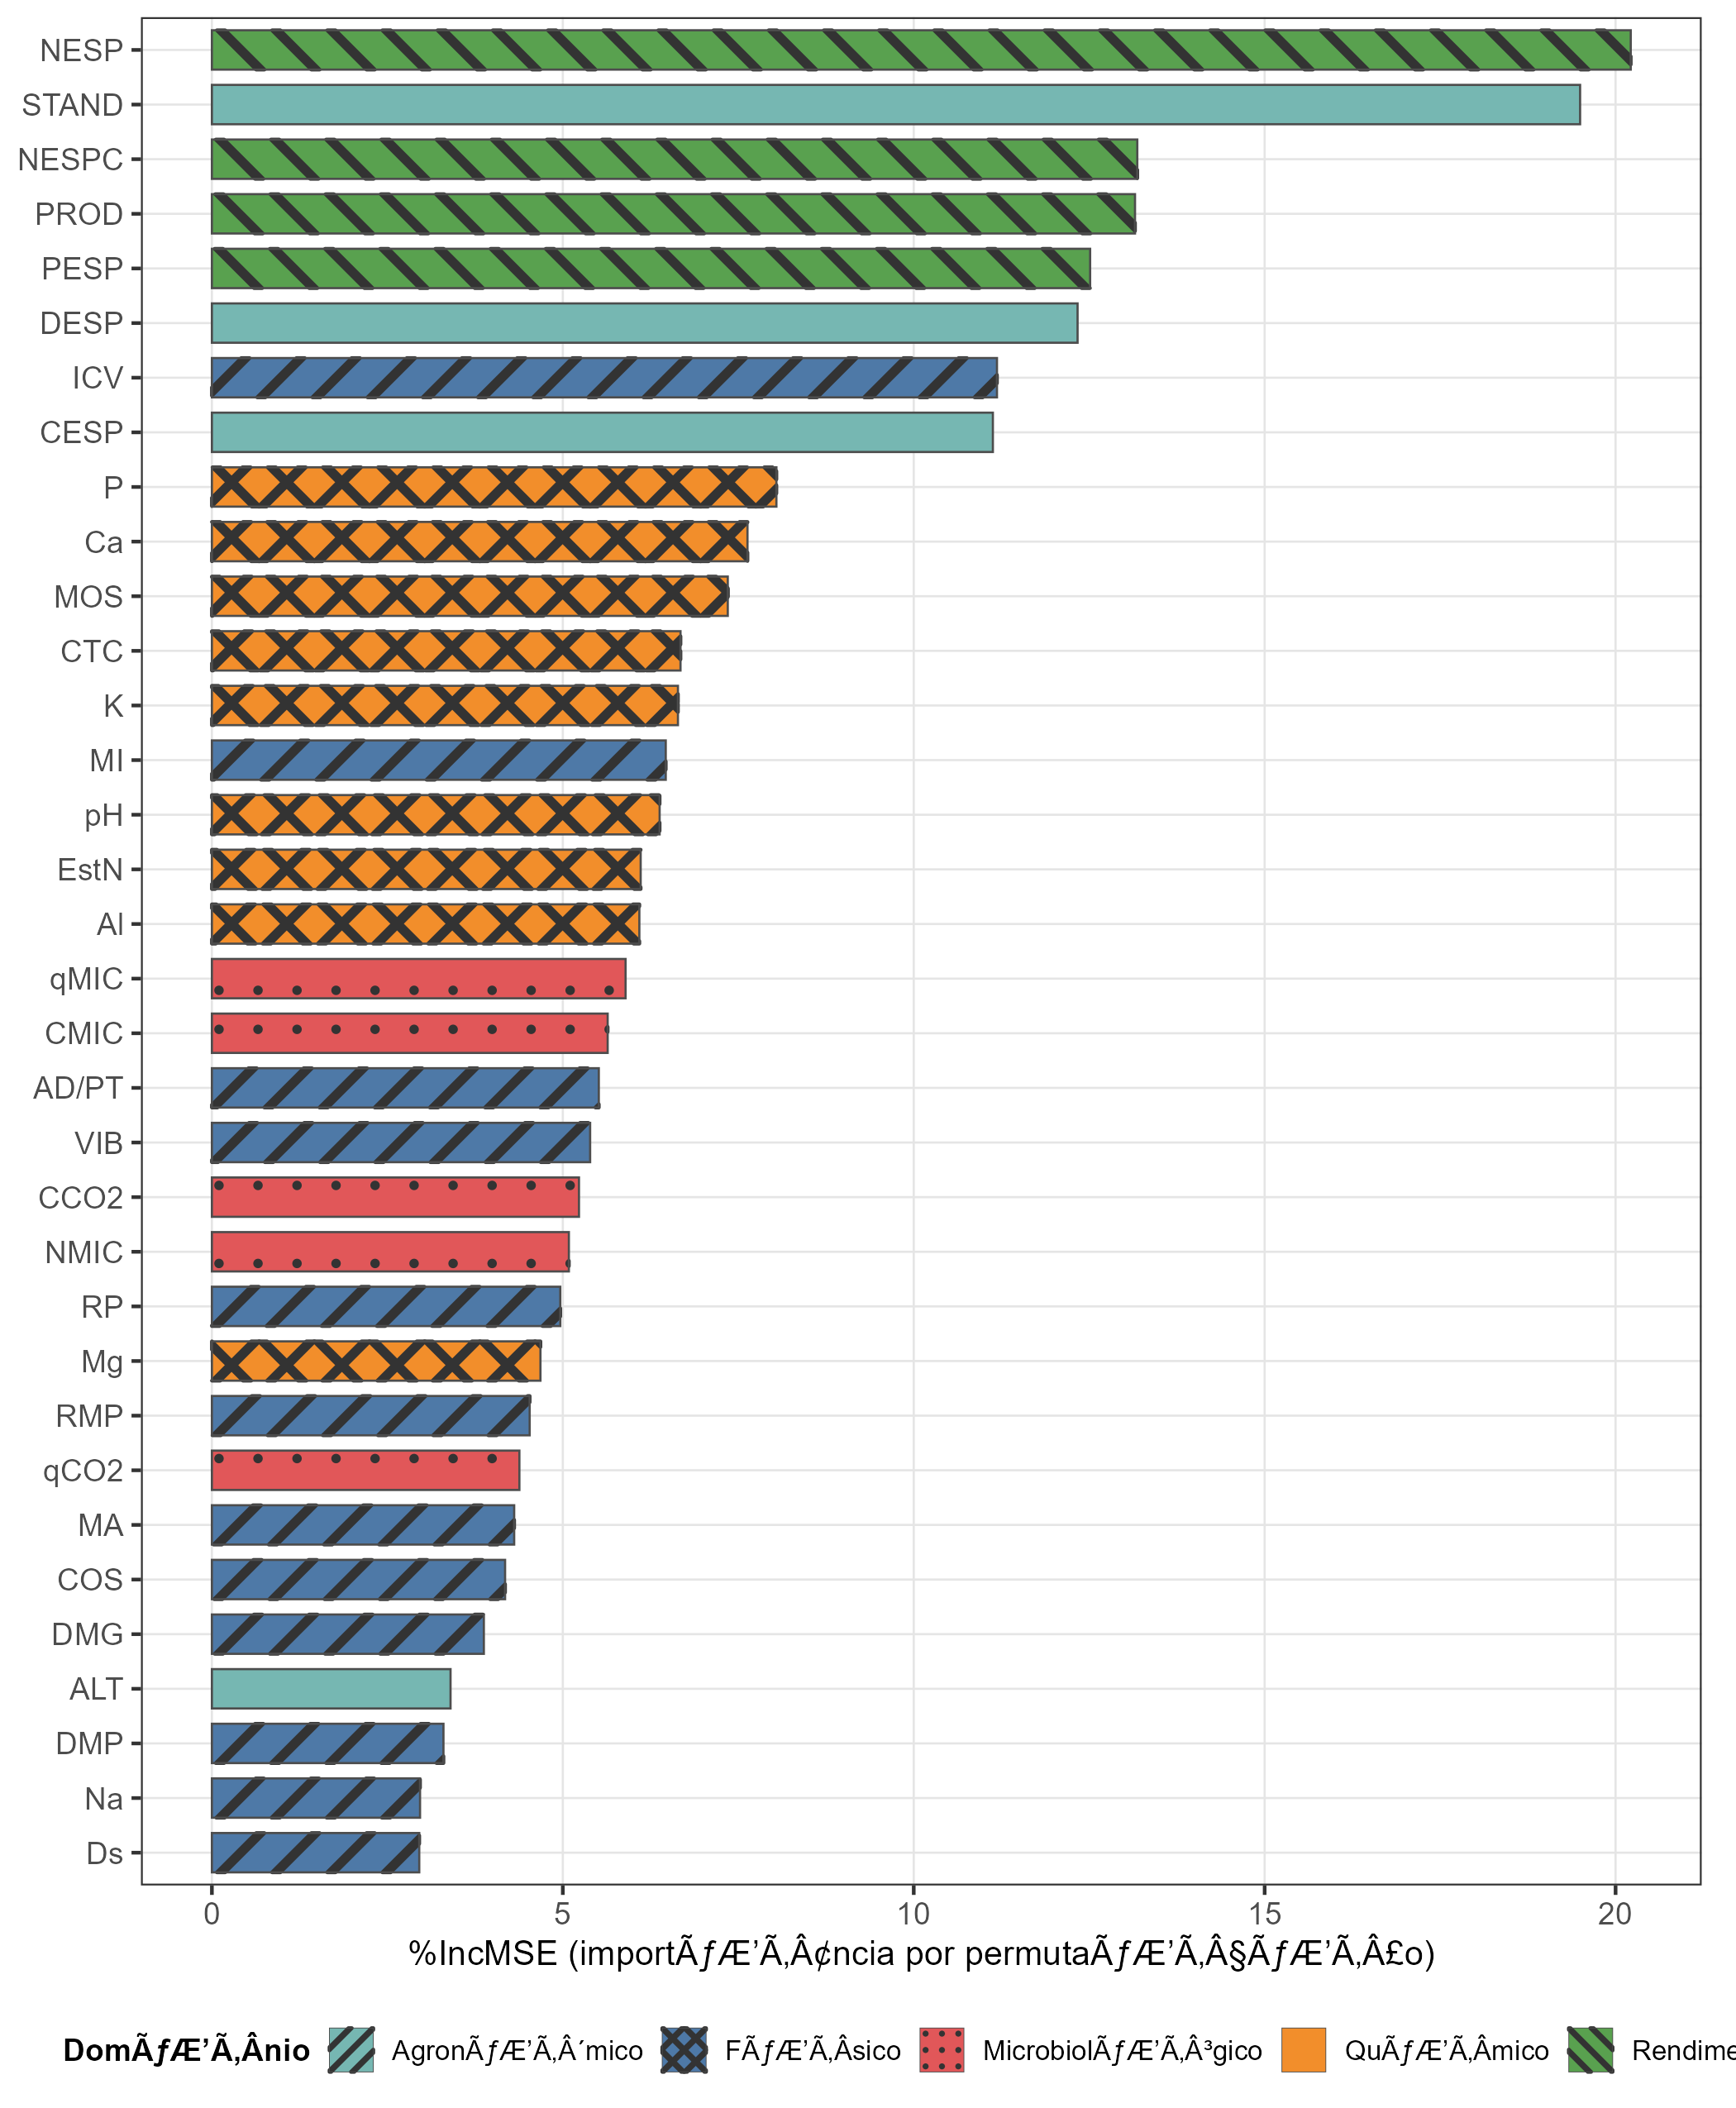
\includegraphics[width=0.75\textwidth]{../../2-DADOS/3-FIGURAS/fig_rf_importance_34.png}
\caption{Importância das variáveis por permutação (\%IncMSE) no modelo RF.}\label{fig:importance}
\smallskip\noindent\textit{Nota:} Barras coloridas por domínio do indicador.
\end{figure}

As curvas de dependência parcial (Fig.~\ref{fig:pdp}) revelam que o número total de espigas por hectare e o estande final exibem resposta sigmoidal sobre o IQS predito pelo RF, com limiar de transição entre os valores normalizados 4 e 6, a partir do qual o efeito marginal se estabiliza em patamar assintótico. O número de espigas comerciais e a produtividade, por sua vez, apresentam resposta monotônica crescente com menor intensidade de saturação, sugerindo contribuição quasi-linear para o escore integrado \citep{Friedman2001}. 

Esse padrão de limiares pode refletir o efeito de compensação entre espécies de cobertura sob Argissolo com camada coesa, em que ganhos de produtividade se estabilizam a partir de determinado nível de estande, enquanto atributos morfológicos mantêm relação de dose-resposta gradual \citep{Assuncao2023}. \cite{Moitinho2020}, ao avaliarem fungos micorrízicos arbusculares sob plantio direto com rotação de milho/cobertura em Argissolo Vermelho, observaram que feijão-guandu e crotalária promoveram maior abundância de esporos e índice de estabilidade de agregados do que gramíneas em monocultura, sugerindo que a mediação biológica da rizosfera pode contribuir para o acoplamento entre qualidade física e resposta produtiva captado pelas PDPs.

\begin{figure}[ht]
\centering
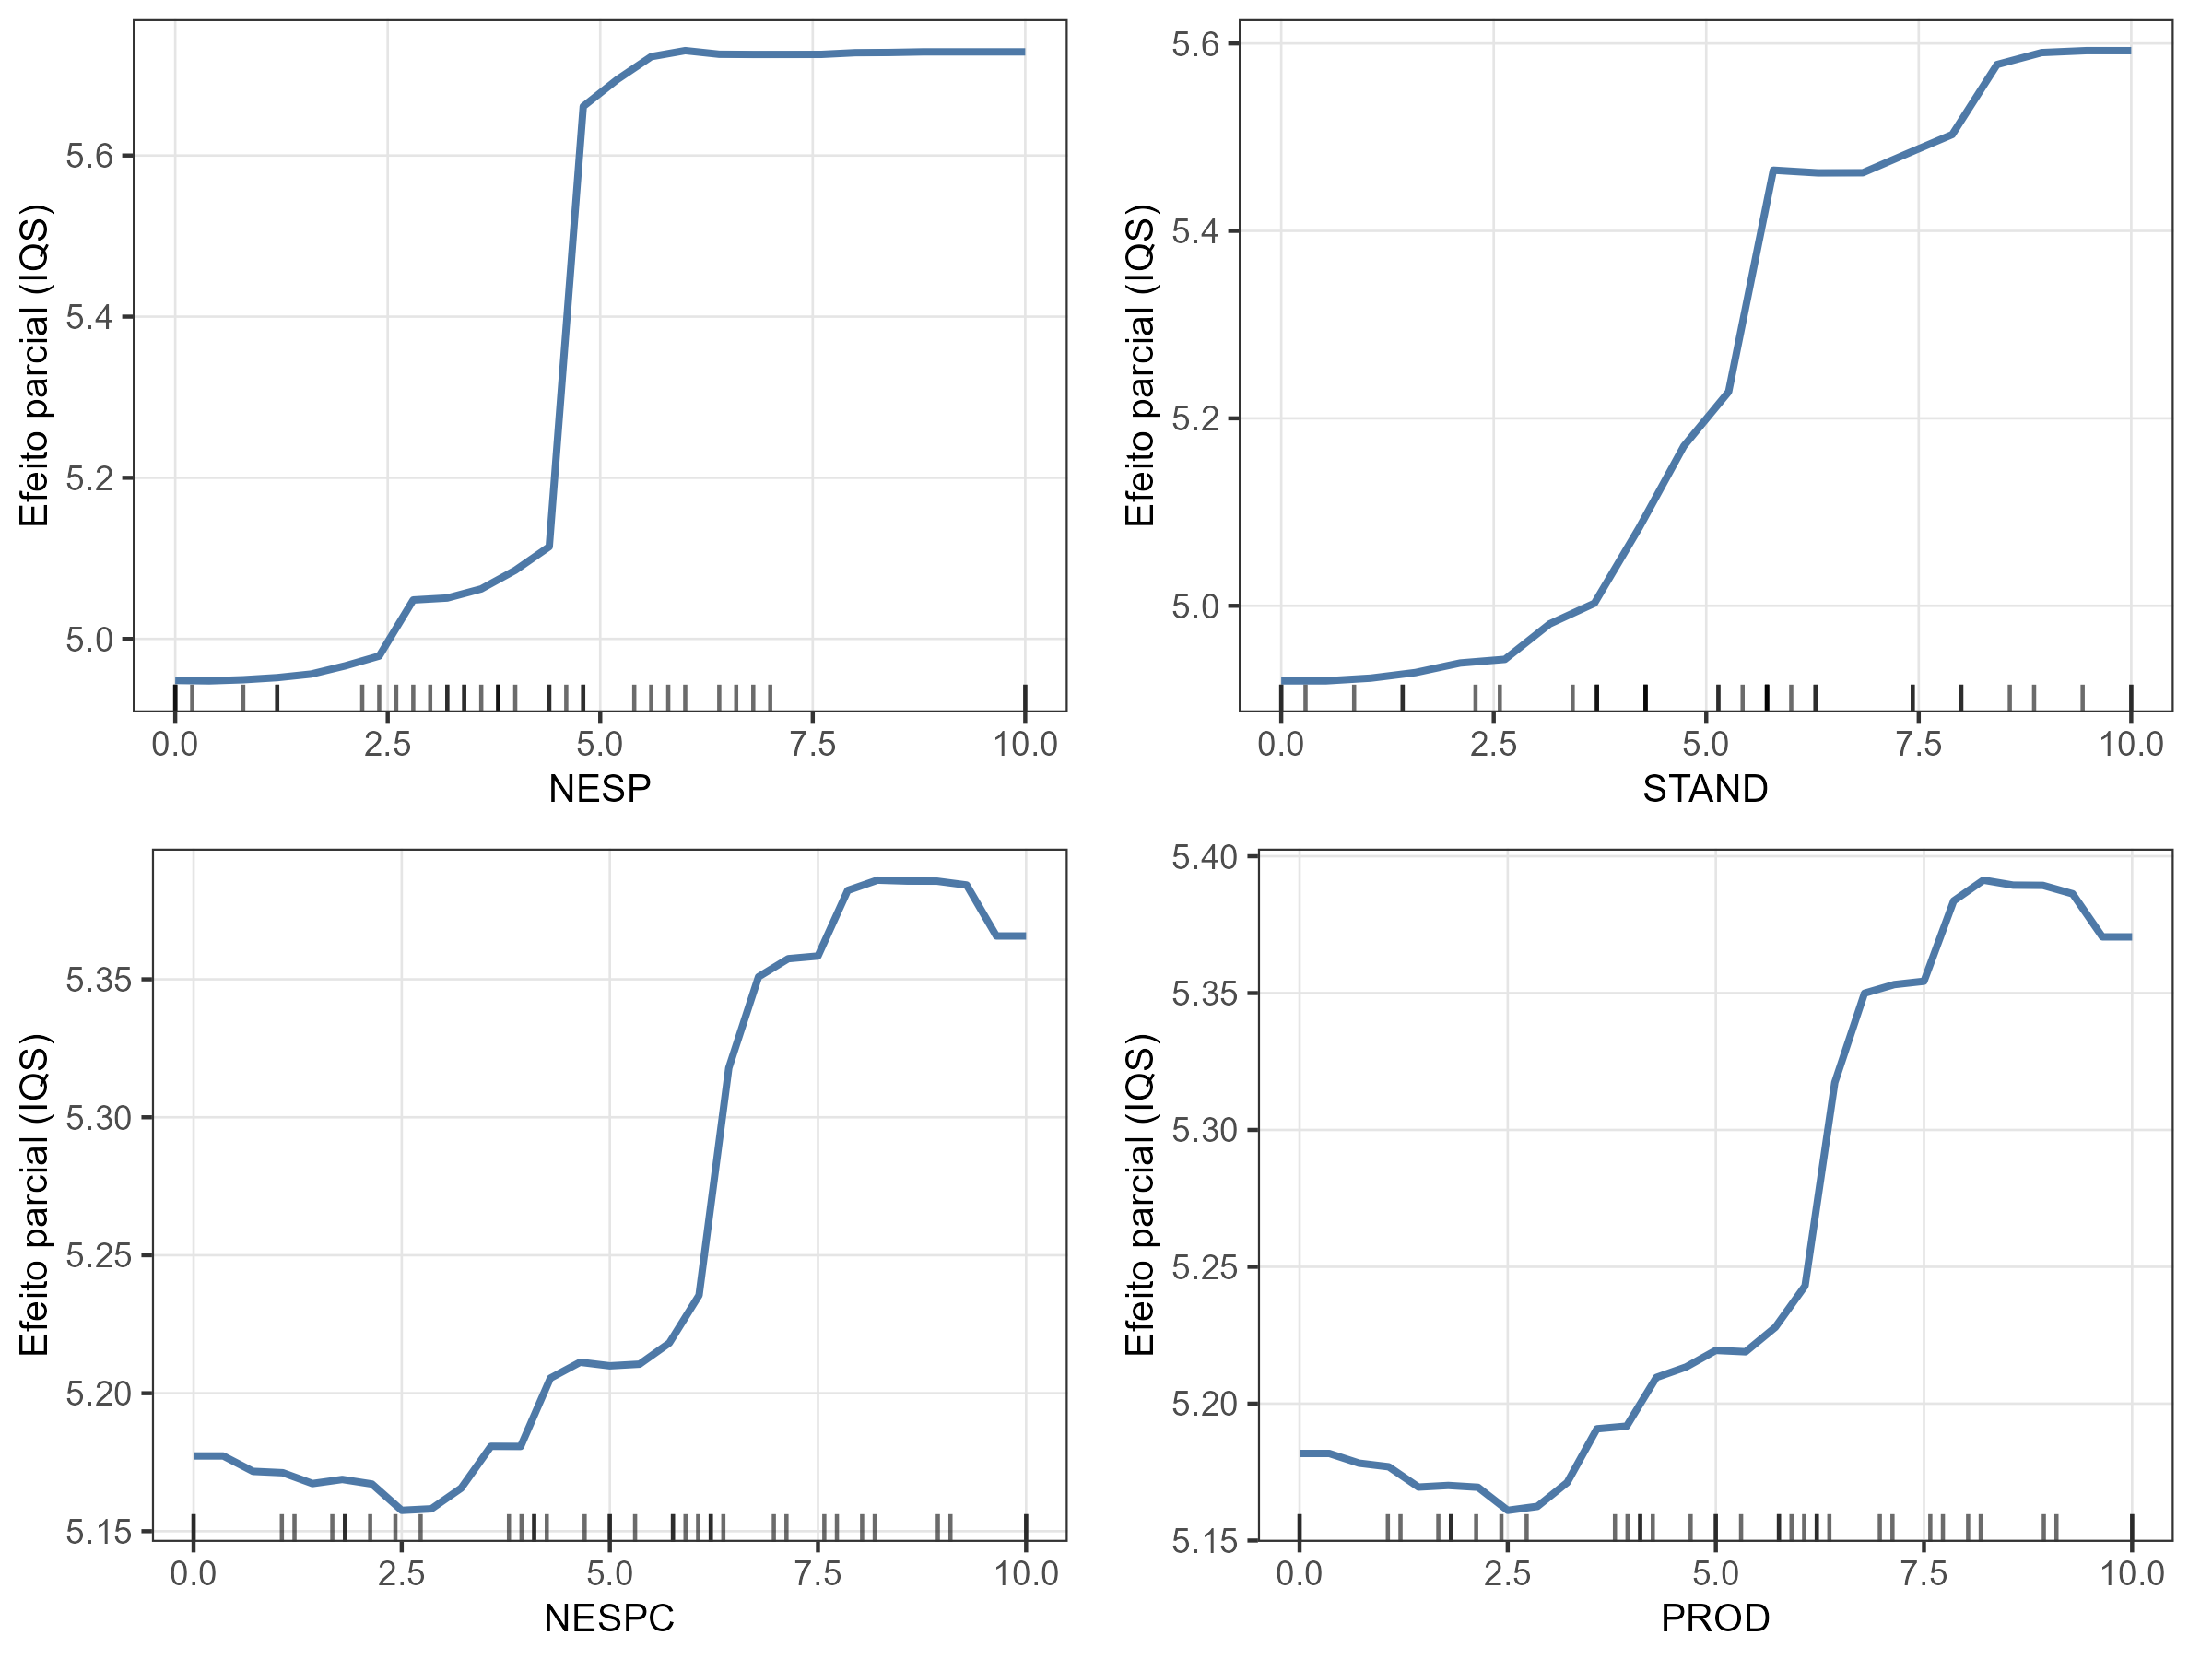
\includegraphics[width=\textwidth]{../../2-DADOS/3-FIGURAS/fig_pdp_top4_34.png}
\caption{Curvas de dependência parcial para os quatro indicadores de maior importância no modelo RF.}\label{fig:pdp}
\smallskip\noindent\textit{Nota:} Eixo horizontal, valor normalizado (0--10); eixo vertical, efeito parcial sobre o IQS predito. \textit{Rug plots} indicam a distribuição marginal dos dados.
\end{figure}

No modelo PLS-SEM com cinco construtos, AGRO explicou a maior parte da variância de REND ($\gamma = 0{,}620$, $p < 0{,}001$), ao passo que os caminhos FISICO$\to$REND ($\gamma = -0{,}132$), QUIMICO$\to$REND ($\gamma = 0{,}086$) e MICRO$\to$REND ($\gamma = -0{,}177$) não atingiram significância estatística. O coeficiente negativo do construto MICRO pode refletir a relação inversa entre atividade microbiana e rendimento imediato frequentemente observada em solos sob aporte contínuo de resíduos, nos quais a imobilização temporária de nutrientes pela biomassa microbiana compete com a absorção radicular \citep{Cardoso2013}. O caminho negativo de FISICO é consistente com a restrição imposta pela camada coesa entre 0,25 e 0,45~m neste Argissolo, que concentra a absorção na camada superficial e pode amplificar correlações negativas aparentes entre indicadores físicos (fortemente condicionados pela restrição subsuperficial) e rendimento. A confirmação desse mecanismo requer amostragem estratificada por profundidade e técnicas de imagem que permitam visualizar a descontinuidade estrutural da camada coesa. 

A triagem por VIF excluiu quatro indicadores (CTC\,=\,37,5; CMIC\,=\,23,9; PROD\,=\,20,1; EstN\,=\,13,7), reduzindo o modelo a 25 variáveis manifestas distribuídas em cinco construtos. O $R^2$ do modelo estrutural para o construto REND foi de 0,688 (Adj.\,$R^2$\,=\,0,676), indicando que os quatro construtos exógenos explicam aproximadamente 69\% da variância do rendimento. O construto de segunda ordem, obtido pelo primeiro componente principal dos cinco escores latentes, foi escalado para o intervalo 0--10 e adotado como IQS$_{\text{PLS}}$.

Os cinco paradigmas produziram distribuições de IQS com amplitude e dispersão distintas. SIF, MARS e RF apresentaram médias próximas (5,24 na escala 0--10, $s \approx 1{,}1$), enquanto o IQS$_{\text{PLS}}$ (média\,$=$\,5,12, $s = 2{,}40$) e o IQS$_{\text{ANOVA}}$ (média\,$=$\,5,10, $s = 2{,}89$) ocuparam faixas mais amplas, reflexo da linearidade e da redução dimensional impostas por esses paradigmas.

\subsection{Concordância inter-paradigma e meta-IQS}\label{subsec:concordance_disc}

O coeficiente de concordância de Kendall ($W = 0{,}726$, $\chi^2 = 389$, $p = 1{,}3 \times 10^{-33}$) indica concordância global significativa entre os cinco ranqueamentos simultâneos \citep{Legendre2012}. O teste de permutação (10\,000 repetições) corroborou esse resultado ($p < 0{,}0001$). O ICC(2,1) de 0,450 (IC\,95\%: 0,360--0,544) indica concordância absoluta moderada, abaixo do limiar de 0,75 geralmente considerado ``bom'' em aplicações de confiabilidade \citep{Koo2016}, refletindo a maior divergência entre famílias analíticas quando indicadores de múltiplos domínios são incluídos. O coeficiente AC1 de Gwet, calculado sobre quintis dos valores de IQS, foi de 0,321 (IC\,95\%: 0,27--0,37), valor conservador que reflete a penalização por concordância marginal esperada ao acaso.

A ampliação do vetor de indicadores de 18 para 34, com a incorporação dos domínios químico expandido e microbiológico, reduziu $W$ de 0,83 para 0,73 e o ICC de 0,74 para 0,45, indicando que a adição de indicadores de múltiplos domínios amplificou a divergência entre paradigmas lineares e não lineares.

A matriz de correlação de Spearman revelou uma estrutura em dois blocos fortemente diferenciados (Tabela~\ref{tab:spearman}). SIF, MARS e RF formaram um bloco quase indistinguível ($\rho > 0{,}992$ entre quaisquer pares), enquanto ANOVA divergiu acentuadamente tanto do bloco não linear ($\rho = 0{,}269$--$0{,}286$) quanto do PLS-SEM ($\rho = 0{,}586$). O PLS-SEM ocupou posição intermediária, com correlações moderadas com o bloco não linear ($\rho = 0{,}718$--$0{,}743$).

O teste de Wilcoxon confirmou que a concordância mútua entre paradigmas não lineares supera a concordância com paradigmas lineares ($W = 18$, $p = 0{,}012$), com a média entre pares não lineares ($\bar{\rho}_{\text{NL-NL}} = 0{,}994$) superando a média entre pares linear--não linear ($\bar{\rho}_{\text{Lin-NL}} = 0{,}502$). Esse resultado indica que a incorporação de indicadores dos domínios químico expandido e microbiológico amplificou a divergência entre famílias analíticas, expondo relações de alta ordem e interações entre domínios que os paradigmas não lineares capturam mas que a decomposição linear por ACP comprime para o resíduo \citep{Zeraatpisheh2020}.

\begin{table}[ht]
\caption{Matriz de correlação de Spearman ($\rho$) entre os cinco paradigmas de IQS após transformação de Blom.}\label{tab:spearman}
\begin{tabular*}{\textwidth}{@{\extracolsep\fill}lccccc}
\toprule
 & ANOVA & Fuzzy & PLS-SEM & MARS & RF \\
\midrule
ANOVA   & 1,000 & 0,269 & 0,586 & 0,276 & 0,286 \\
Fuzzy   &       & 1,000 & 0,723 & 0,994 & 0,994 \\
PLS-SEM &       &       & 1,000 & 0,718 & 0,743 \\
MARS    &       &       &       & 1,000 & 0,992 \\
RF      &       &       &       &       & 1,000 \\
\botrule
\end{tabular*}
\end{table}

Os limites de concordância de Bland--Altman \citep{BlandAltman1986} (Tabela~\ref{tab:blandaltman}) reforçaram quantitativamente essa estrutura em dois blocos. Os LoA entre pares do bloco SIF-MARS-RF variaram de $\pm 0{,}35$ (Fuzzy vs.\ MARS) a $\pm 0{,}41$ (MARS vs.\ RF) na escala Blom, sugerindo substituibilidade prática. Em contraste, os pares envolvendo ANOVA apresentaram LoA de $\pm 1{,}80$ (ANOVA vs.\ PLS) a $\pm 2{,}40$ (ANOVA vs.\ Fuzzy), ao passo que PLS-SEM versus bloco não linear situou-se em faixa intermediária (LoA $\approx \pm 1{,}58$), indicando que a substituição do paradigma linear por qualquer alternativa não linear pode alterar posições de ranqueamento individuais.

\begin{table}[ht]
\caption{Sumário da análise de Bland--Altman entre pares de paradigmas (escala Blom).}\label{tab:blandaltman}
\begin{tabular*}{\textwidth}{@{\extracolsep\fill}lcccc}
\toprule
Par & $\overline{\Delta M}$ & $s_{\Delta M}$ & LoA inf. & LoA sup. \\
\midrule
Fuzzy vs RF    & 0,00 & 0,206 & $-$0,403 & 0,403 \\
Fuzzy vs MARS  & 0,00 & 0,181 & $-$0,353 & 0,357 \\
MARS vs RF     & 0,00 & 0,206 & $-$0,406 & 0,402 \\
PLS vs Fuzzy   & 0,00 & 0,817 & $-$1,601 & 1,601 \\
PLS vs MARS    & 0,00 & 0,805 & $-$1,576 & 1,580 \\
PLS vs RF      & 0,00 & 0,804 & $-$1,575 & 1,575 \\
ANOVA vs PLS   & 0,00 & 0,918 & $-$1,800 & 1,800 \\
ANOVA vs Fuzzy & 0,00 & 1,226 & $-$2,403 & 2,403 \\
ANOVA vs MARS  & 0,00 & 1,203 & $-$2,356 & 2,360 \\
ANOVA vs RF    & 0,00 & 1,207 & $-$2,365 & 2,365 \\
\botrule
\end{tabular*}
\smallskip\noindent\textit{Nota:} $\overline{\Delta M}$, diferença média; $s_{\Delta M}$, desvio-padrão da diferença; LoA, limites de concordância ($\pm 1{,}96\,s_{\Delta M}$).
\end{table}

\clearpage

A substituibilidade prática dentro do bloco não linear é confirmada pela dispersão homogênea do par Fuzzy--RF na faixa $\pm 0{,}40$ ao longo do eixo de médias, com pontos distribuídos simetricamente em torno da diferença nula e sem tendência proporcional ao nível do IQS. O par ANOVA--Fuzzy, em contraste, apresenta padrão em leque que sugere viés proporcional ao nível do IQS \citep{Giavarina2015}, com discordância crescente em direção aos valores mais elevados da escala Blom e LoA de $\pm 2{,}40$, o que indica que a compressão linear diverge progressivamente dos paradigmas não lineares à medida que o escore integrado se eleva. 

O par PLS--RF ocupa posição intermediária (LoA\,$\approx \pm 1{,}58$), com aparente heteroscedasticidade nos valores extremos que sinaliza discordância mais acentuada para combinações de manejo com qualidade inferior (Fig.~\ref{fig:ba_panel}). Esse gradiente de concordância, da substituibilidade do bloco não linear à divergência sistemática dos paradigmas lineares, reforça que a escolha da família analítica, e não apenas a parametrização interna de cada algoritmo, governa o grau de concordância entre ranqueamentos de IQS.

\begin{figure}[ht]
\centering
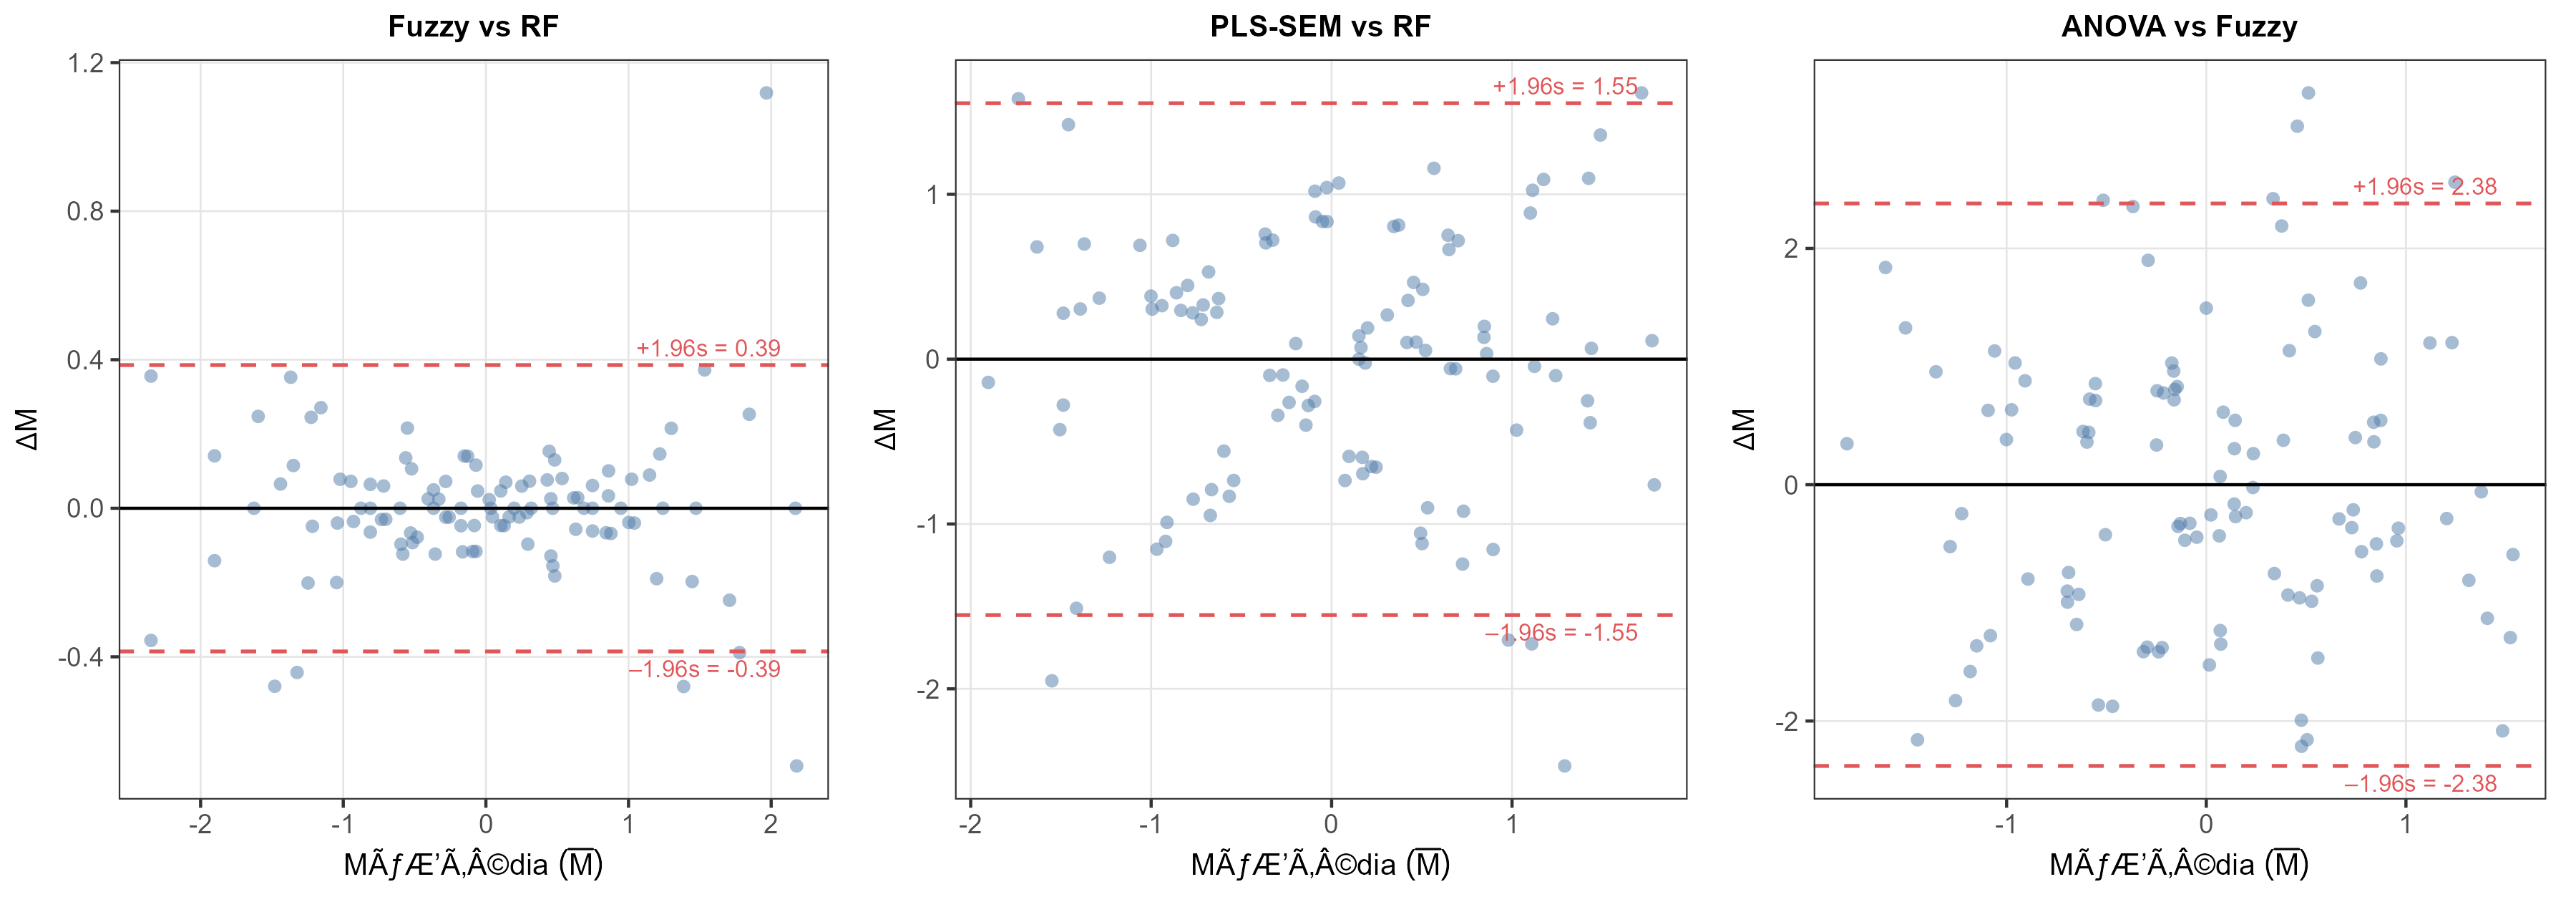
\includegraphics[width=\textwidth]{../../2-DADOS/3-FIGURAS/fig_blandaltman_panel_34.png}
\caption{Diagramas de Bland--Altman para três pares representativos de paradigmas (escala Blom).}\label{fig:ba_panel}
\smallskip\noindent\textit{Nota:} Linha contínua, diferença média ($\overline{\Delta M} \approx 0$); linhas tracejadas, limites de concordância a $\pm 1{,}96\,s_{\Delta M}$.
\end{figure}

A proximidade com a diagonal de identidade varia entre paradigmas nos diagramas de dispersão 1:1 (Fig.~\ref{fig:scatter1to1}). Fuzzy ($\rho^2 = 0{,}989$) e MARS ($\rho^2 = 0{,}984$) alinham-se quase perfeitamente, ao passo que PLS-SEM ($\rho^2 = 0{,}552$) e ANOVA ($\rho^2 = 0{,}082$) apresentam dispersão pronunciada, com observações individuais desviando em até 2,0 unidades Blom da reta 1:1 \citep{Venkateswarlu2025}.

\begin{figure}[ht]
\centering
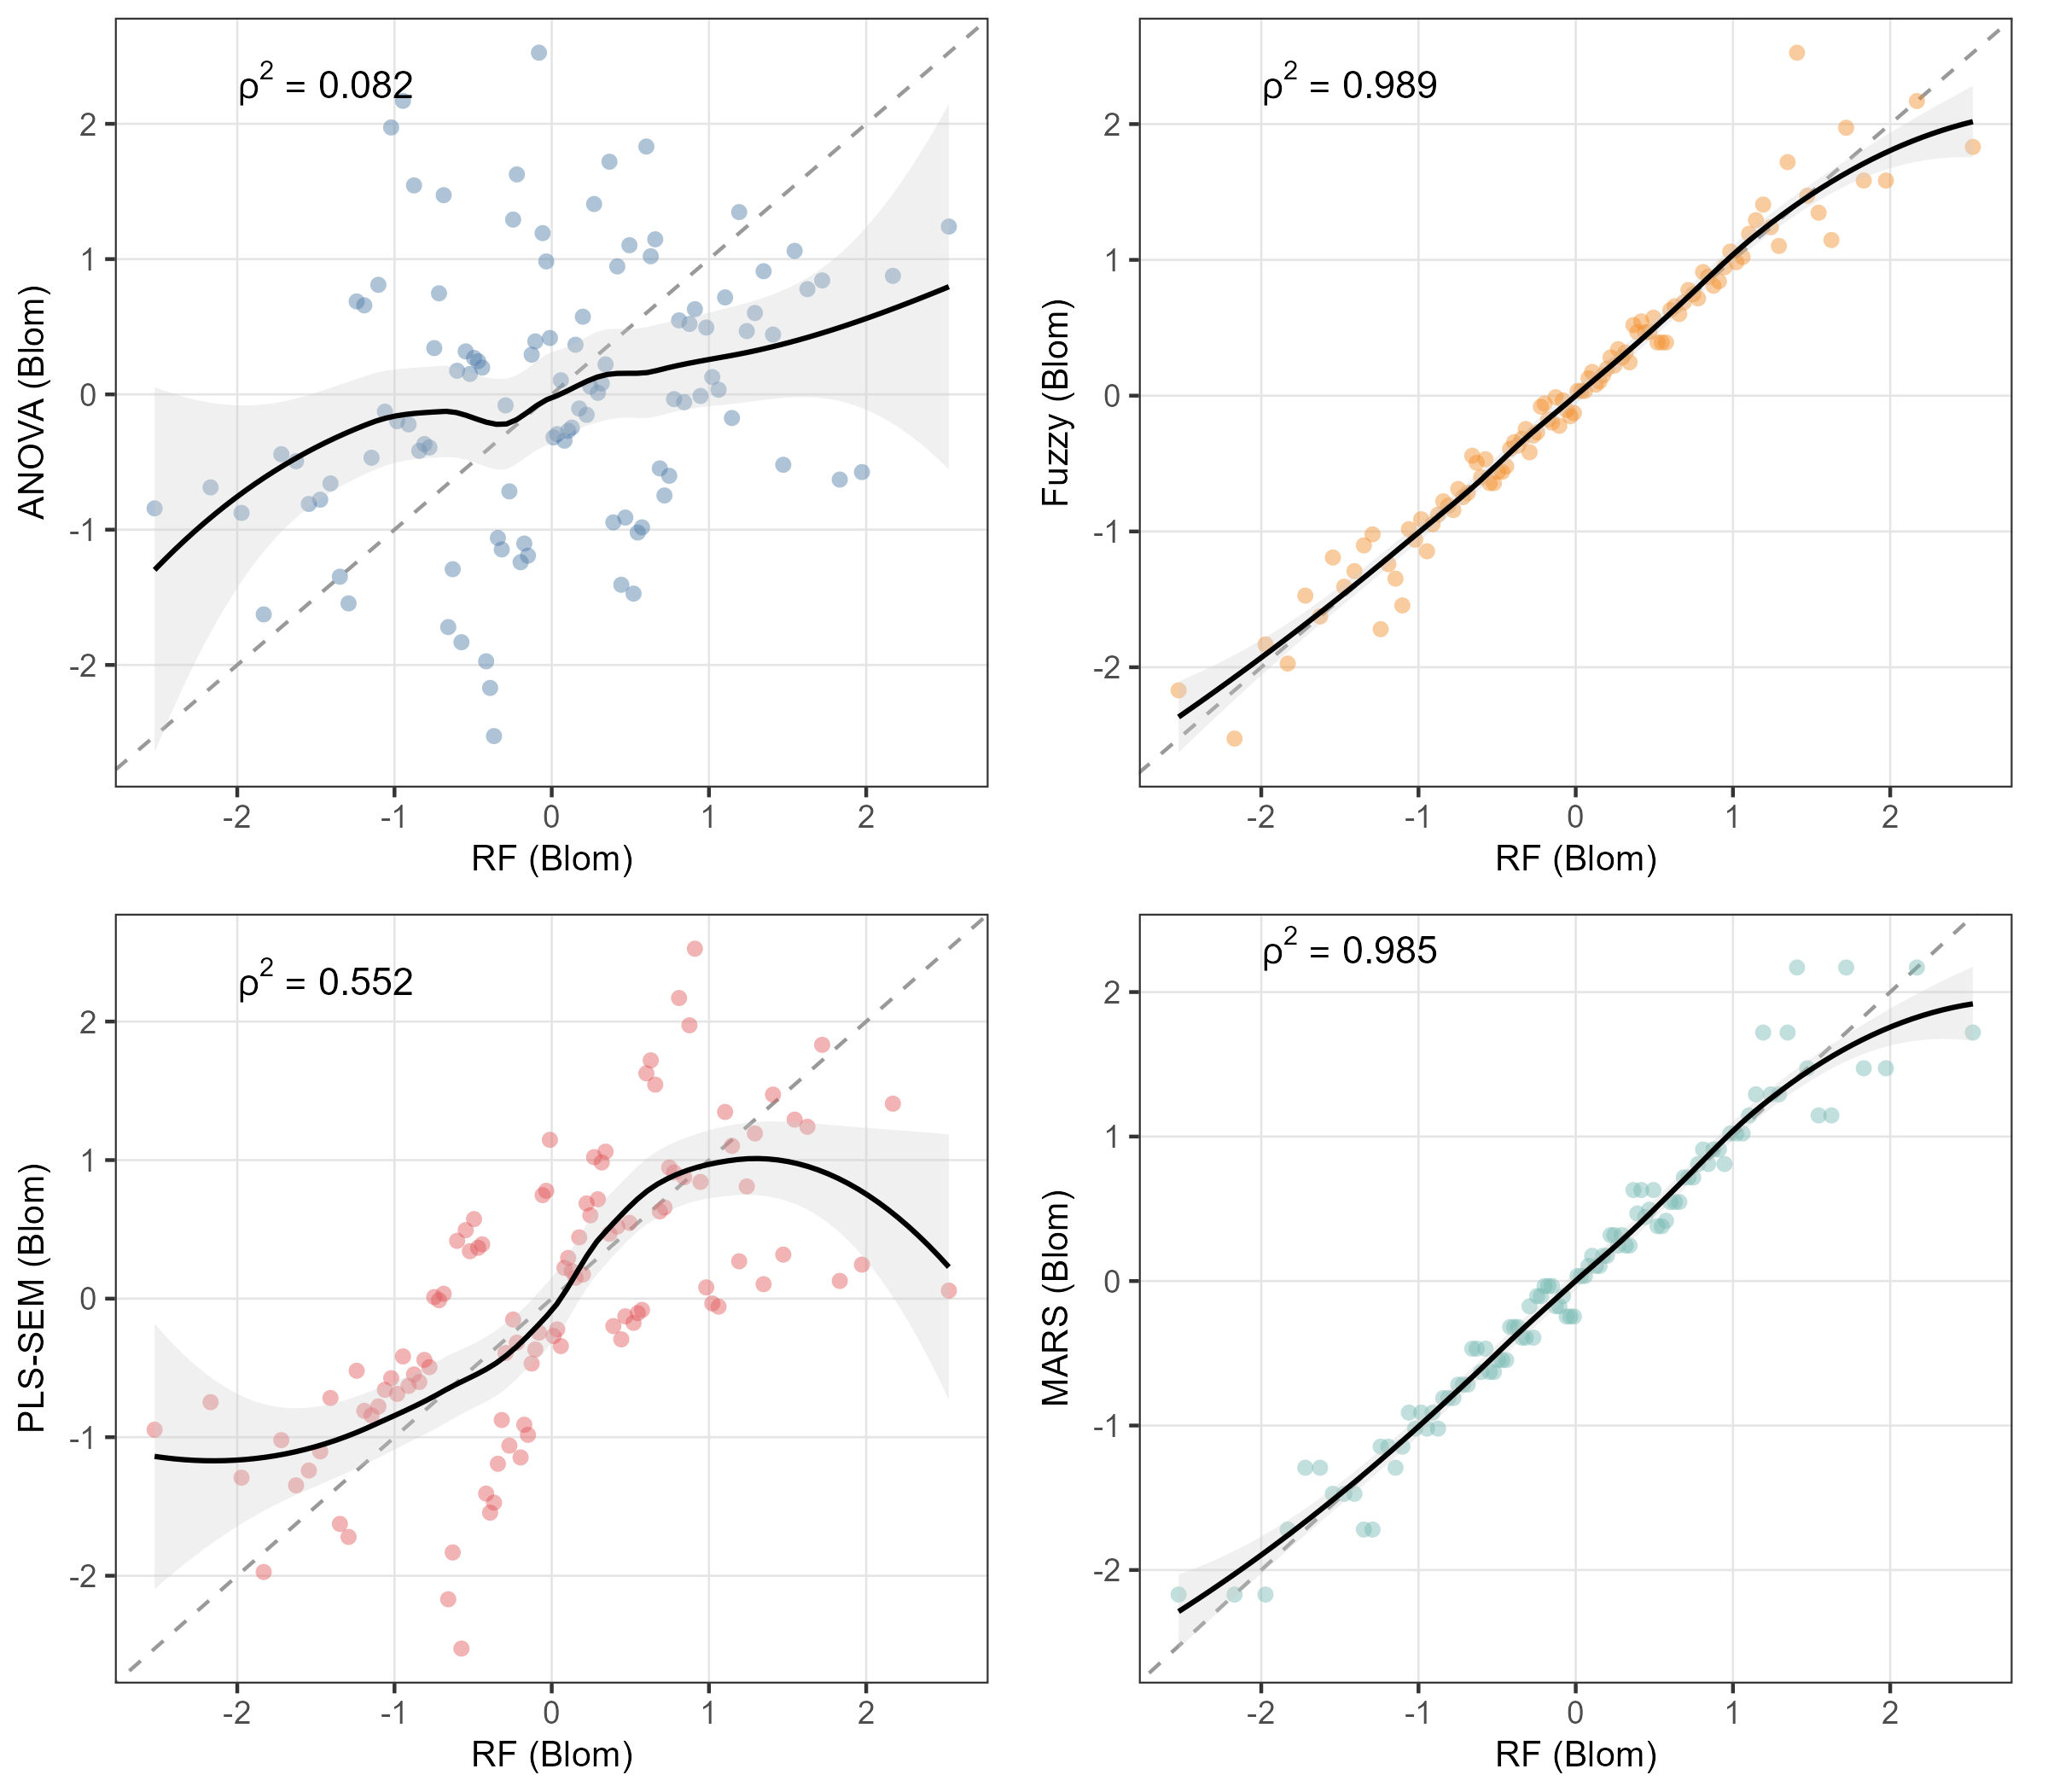
\includegraphics[width=\textwidth]{../../2-DADOS/3-FIGURAS/fig_scatter_1to1_34.png}
\caption{Diagramas de dispersão 1:1 de IQS (escala Blom) entre cada paradigma e o RF como referência.}\label{fig:scatter1to1}
\smallskip\noindent\textit{Nota:} Linha tracejada, identidade; linha contínua, regressão local. Valores de $\rho^2$ anotados em cada painel.
\end{figure}

Essa magnitude de desvio implica que, para uma dada observação, o diagnóstico de qualidade ``alta'' ou ``baixa'' pode ser contingente ao paradigma quando se adota o limiar convencional da mediana, padrão que reforça a necessidade de métricas de concordância na avaliação de IQS \citep{Liu2025}. \cite{Kahsay2025}, ao compararem oito modelos de IQS (TDS/MDS $\times$ escore linear/não linear $\times$ IQI/NQI) em terras degradadas da Etiópia, verificaram que a função de escore não linear produziu índices sistematicamente 12--18\% superiores ao escore linear, com divergência amplificada em solos de baixa qualidade, padrão consistente com o viés em leque entre ANOVA e Fuzzy observado neste estudo (Fig.~\ref{fig:ba_panel}). \cite{Zhang2024LDD}, em rotação trigo--milho sob plantio convencional e conservacionista no norte da China, reportaram que o IQS com escore não linear detectou benefícios do manejo conservacionista que o escore linear não distinguiu, o que reforça a hipótese de que a família analítica, e não apenas o conjunto de indicadores, condiciona a sensibilidade do índice.

A convergência entre SIF, MARS e RF é consistente com a hipótese de que esses paradigmas acessam o mesmo subespaço de variabilidade, definido por relações não lineares e interações de alta ordem entre indicadores que o modelo linear comprime ou ignora \citep{Zeraatpisheh2020,Wadoux2020}. \cite{DosSantos2021} observaram padrão análogo em Latossolo Vermelho sob sistemas integrados de produção, com o IQS fuzzy detectando diferenças de manejo que o protocolo aditivo clássico não distinguiu, o que sustenta a generalidade da convergência não linear em solos tropicais.

A ampliação do vetor de indicadores de 18 para 34, com a incorporação dos domínios químico expandido e microbiológico, intensificou a diferenciação entre famílias analíticas, reduzindo o $\bar{\rho}_{\text{Lin-NL}}$ de 0,71 para 0,50 e tornando significativa a divergência entre famílias analíticas ($p = 0{,}012$). Esse resultado indica que os indicadores microbiológicos e químicos adicionais introduziram variância entre-parcelas com estrutura predominantemente não linear, que os algoritmos adaptativos capturam como interações de alta ordem entre domínios, ao passo que a ACP projeta essa informação sobre componentes ortogonais que comprimem as relações inter-domínio \citep{Rezaee2020}.

A amplitude dessa discordância varia com o tipo de solo e com o método de indexação. Divergências de até 30\% entre índices aditivos ponderados e cumulativos foram reportadas em solos com distribuição heterogênea de indicadores no Irã central \citep{Emami2024}, magnitude consistente com os LoA de $\pm 1{,}80$ a $\pm 2{,}40$ observados neste estudo para pares envolvendo a ANOVA. Em solos costeiros salinos da Índia, a concordância entre três métodos (SQI$_w$ aditivo, SQI$_n$ Nemoro e SQI$_c$ cumulativo) variou com a severidade da salinidade, sendo mais elevada em solos de qualidade intermediária e menor nos extremos \citep{Mahajan2021}, padrão que se assemelha à heteroscedasticidade documentada nos diagramas de Bland--Altman deste estudo.

O PLS-SEM, por especificar caminhos lineares entre construtos latentes mas incorporar indicadores formativos (Mode~B) que capturam parcialmente a não linearidade na composição \citep{Diamantopoulos2008}, convergiu com o bloco não linear ($\rho = 0{,}72$--$0{,}74$) mais do que a ANOVA ($\rho = 0{,}27$--$0{,}29$), com LoA de $\pm 1{,}58$ que são inferiores aos LoA da ANOVA ($\pm 2{,}40$). A divergência acentuada da ANOVA ($\rho \approx 0{,}28$ com o bloco NL) é consistente com a dependência de pesos derivados de ACP e de combinação linear de escores ortogonais, que perdem informação sobre interações de ordem superior \citep{Andrews2002,Bünemann2018}, indicando que a substituibilidade entre paradigmas depende da família analítica, e não do algoritmo específico.

Comparações anteriores entre métodos de IQS já haviam sugerido que a ordenação extrema tende a ser preservada mesmo quando os escores absolutos divergem em até 15\% \citep{Mukherjee2014}, porém essas comparações permaneceram restritas a variantes de uma mesma família algorítmica \citep{Chaudhry2024} ou careceram de protocolo formal de concordância inter-avaliador \citep{Pacci2026}. A confrontação simultânea de cinco famílias com pressupostos estruturalmente distintos, associada a métricas de concordância ($W$, ICC, Bland--Altman), permitiu quantificar limiares de substituibilidade ($\rho > 0{,}99$ e LoA\,$< \pm 0{,}41$ para o bloco SIF-MARS-RF) que podem servir como referência em futuros exercícios de benchmarking de IQS \citep{Cherubin2016}.

A agregação ordinal por contagem de Borda, reconhecida como estratégia para consolidar ranqueamentos divergentes em indicadores compostos \citep{Munda2012}, gerou um meta-IQS com correlação de Spearman $\geq 0{,}95$ em relação aos paradigmas SIF, MARS e RF, patamar consistente com intercambialidade funcional segundo critérios de concordância inter-avaliadores \citep{Gwet2014}, ao passo que a concordância com PLS-SEM ($\rho = 0{,}83$) e ANOVA ($\rho = 0{,}84$) permaneceu em faixa moderada.

A interpretação dos LoA seguiu o critério de \cite{BlandAltman1999}, segundo o qual dois métodos podem ser considerados intercambiáveis quando os limites de concordância são agronomicamente irrelevantes. Pares com $\rho > 0{,}99$ e LoA\,$< \pm 0{,}41$ satisfazem esse critério para ranqueamento de manejo, ao passo que pares com $\rho \approx 0{,}28$ e LoA\,$\approx \pm 2{,}40$ podem produzir divergências em posições intermediárias e mesmo nos extremos. Pares com $\rho \approx 0{,}72$ (PLS vs.\ bloco NL, LoA\,$\approx \pm 1{,}58$) representam concordância moderada que pode ser suficiente quando a prioridade é interpretação causal entre domínios edáficos.

A magnitude dos LoA entre famílias lineares e não lineares ($\approx \pm 1{,}70$ na escala Blom) implica risco operacional para recomendações de manejo baseadas em posições intermediárias do ranqueamento. Das 12 combinações manejo--cobertura avaliadas, seis (50\%) trocaram de faixa de classificação (terço superior $\leftrightarrow$ terço intermediário) quando o paradigma foi substituído de ANOVA para RF, o que pode alterar a priorização de práticas em contextos de extensão rural.

O custo de uma recomendação equivocada pode ser estimado pelo diferencial de rendimento entre combinações adjacentes no ranqueamento. Adotar PC-Caupi (posição 4 pelo RF, posição 8 pela ANOVA) em lugar de CM-Crotalária (estável na 2\textsuperscript{a}--4\textsuperscript{a} posição) pode representar perda de rendimento da ordem de 15--20\% na produção de milho verde \citep{SantosJA2024}, equivalente a aproximadamente 1\,200--1\,800\,kg\,ha$^{-1}$ de espigas comerciais no contexto dos Tabuleiros Costeiros. Essa magnitude sugere que a escolha do paradigma não é neutra do ponto de vista econômico e pode justificar a inclusão de análise de sensibilidade inter-paradigma em avaliações de IQS destinadas a subsidiar políticas de conservação do solo.

\subsection{Ranqueamento por combinação manejo--cobertura}\label{subsec:ranking}

A distribuição dos escores de IQS por combinação manejo--cobertura (Fig.~\ref{fig:boxplot_combo}) evidencia que o cultivo mínimo com feijão-guandu (CM-Guandu) concentrou os maiores valores medianos para todos os cinco paradigmas, com amplitudes interquartílicas reduzidas que sugerem baixa variabilidade interna nessa combinação. Com comportamento oposto, plantio convencional com feijão-guandu (PC-Guandu) exibiu os escores mais baixos em todos os paradigmas, com medianas próximas de 1,0 na escala original. O desempenho comparativamente superior do cultivo mínimo com guandu, já reportado por \cite{Assuncao2023} para o 17\textsuperscript{o} ano deste mesmo experimento, sugere persistência temporal do efeito de manejo ao longo de pelo menos cinco safras adicionais, resultado que pode refletir a interação entre a fixação biológica de nitrogênio do guandu e a magnitude do revolvimento mecânico aplicado.

\begin{figure}[ht]
\centering
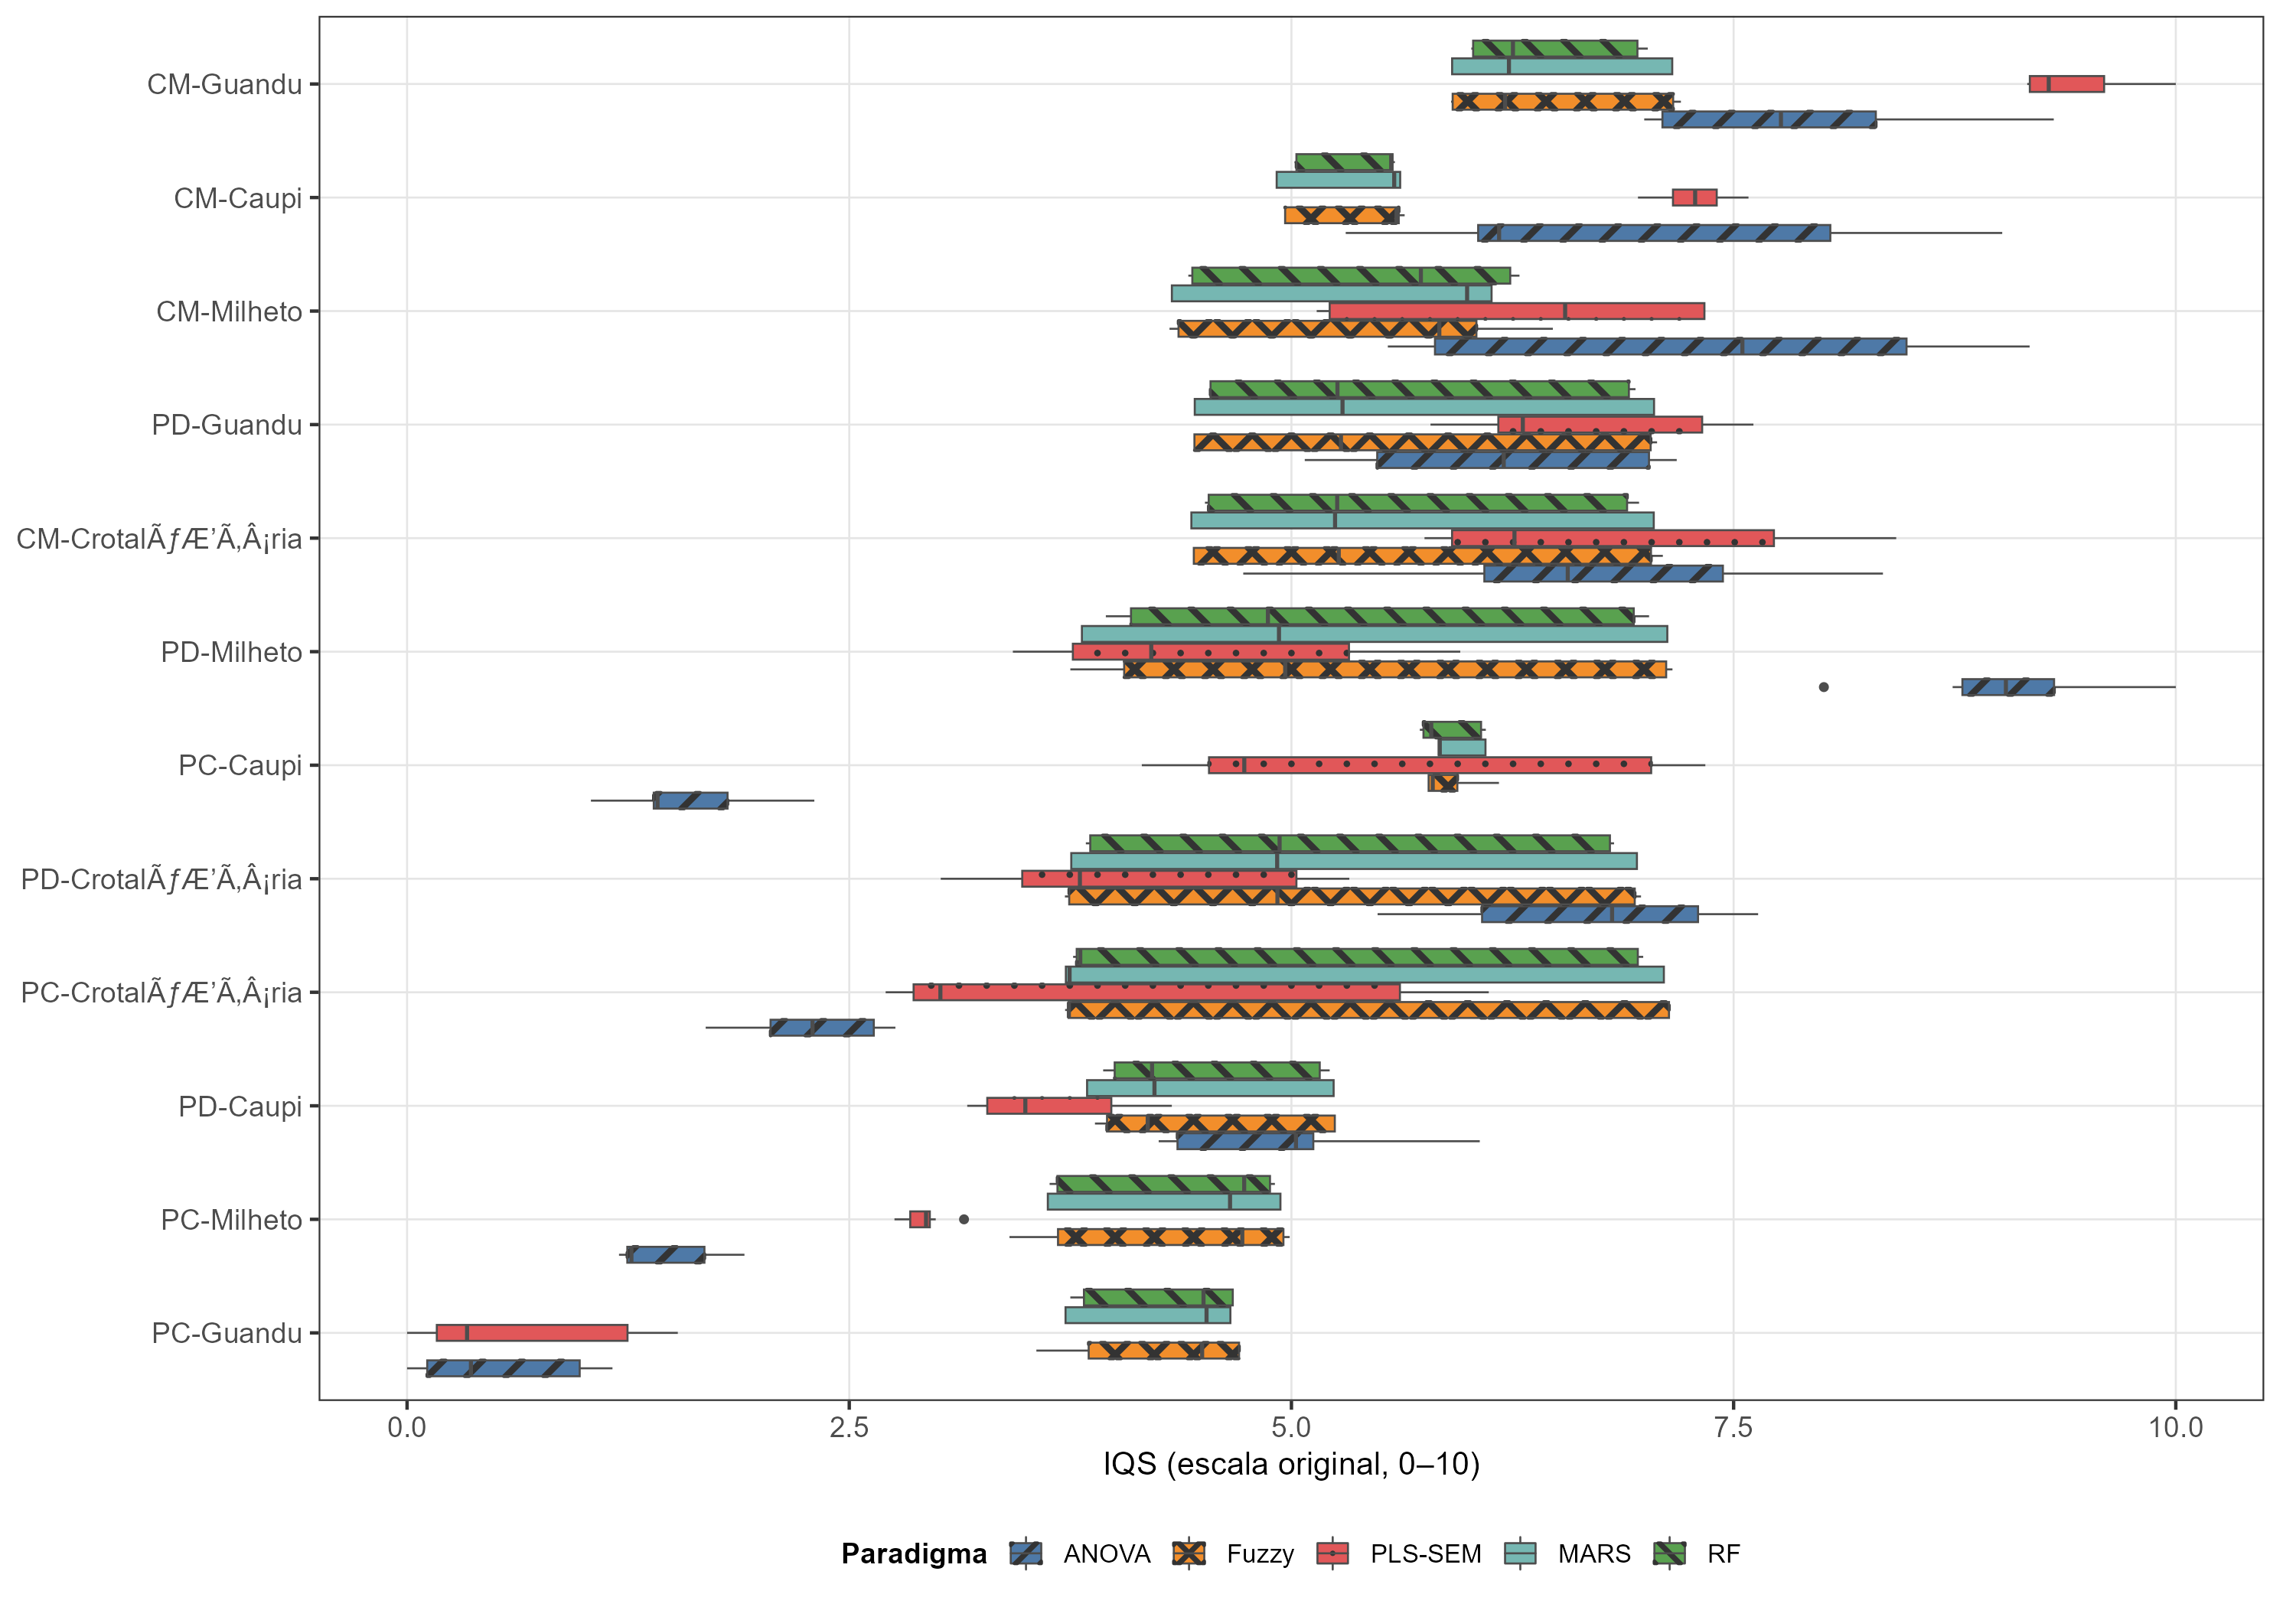
\includegraphics[width=\textwidth]{../../2-DADOS/3-FIGURAS/fig_boxplot_combo_34.png}
\caption{Distribuição do IQS (escala original, 0--10) por combinação manejo--cobertura e paradigma analítico.}\label{fig:boxplot_combo}
\smallskip\noindent\textit{Nota:} Combinações ordenadas pela média do meta-IQS de Borda.
\end{figure}
 Ao avaliarem a produção de milho verde nas mesmas parcelas de longa duração no Nordeste brasileiro, \cite{SantosJA2024} observaram que o cultivo mínimo associado a plantas de cobertura produziu rendimentos 28\% superiores ao plantio convencional, com o guandu contribuindo para ruptura parcial da camada coesa pelo sistema radicular pivotante profundo ($> 2$~m). 

Esse mecanismo é consistente com observações de \cite{daSilva2021}, que verificaram em Argissolo Vermelho sob plantio direto que a sucessão milho/crotalária promoveu índice de estabilidade de agregados ($> 90$\%) superior à sucessão milho/pousio, atribuindo a diferença à glomalina e ao aporte contínuo de matéria orgânica particulada na rizosfera de leguminosas.

O posicionamento do plantio convencional com guandu na última posição de todos os cinco paradigmas (Borda\,=\,18,2) sugere um paradoxo aparente que o mecanismo de destruição estrutural pode explicar. O revolvimento por aração a 25\,cm seguida de gradagem rompe as redes de hifas fúngicas e os bioporos contínuos (diâmetro $> 75$\,\textmu m) criados pelo sistema radicular pivotante do guandu, anulando os benefícios de fixação biológica de N$_2$ (50--200\,kg\,N\,ha$^{-1}$\,ano$^{-1}$) e de ruptura da camada coesa \citep{Peoples2009}. 

Essa desconexão entre aporte de N e preservação estrutural explica por que a mesma espécie de cobertura ocupa simultaneamente a primeira (CM-Guandu) e a última (PC-Guandu) posição do ranqueamento, uma vez que o benefício agronômico da leguminosa é condicionado pela manutenção da integridade física do solo. \cite{Thomaz2022}, em experimento de 23 anos com tabaco no sul do Brasil, documentaram redução de 45\% no índice de estabilidade de agregados e incremento de erodibilidade ($K$-USLE de 0,018 para 0,031~Mg ha h ha$^{-1}$ MJ$^{-1}$ mm$^{-1}$) em plantio convencional comparado ao plantio direto, corroborando que o revolvimento mecânico reiterado sobrepõe-se ao efeito rizosférico da leguminosa.

As posições intermediárias, contudo, apresentaram inversões entre paradigmas em 67\% das combinações manejo--cobertura (8 de 12). PC-Caupi ocupou a 2\textsuperscript{a} posição por Fuzzy, MARS e RF, porém a 10\textsuperscript{a} pela ANOVA, configurando a maior inversão observada (8 posições). PD-Milheto exibiu padrão simétrico, alcançando a 1\textsuperscript{a} posição pela ANOVA e a 7\textsuperscript{a} por todos os paradigmas não lineares e pelo PLS-SEM. CM-Crotalária ascendeu à 3\textsuperscript{a} posição no PLS-SEM, mas posicionou-se na 4\textsuperscript{a} por Fuzzy e MARS. 

Essa inversão é consistente com a sensibilidade diferencial dos paradigmas à contribuição relativa dos indicadores físicos versus de rendimento, uma vez que o protocolo MDS da ANOVA aplica pesos derivados de ACP que equalizam domínios, enquanto os paradigmas não lineares ponderam pela capacidade preditiva estimada pelo algoritmo \citep{Chaudhry2024}. \cite{Fernandes2022}, em estudo sobre agregação em plantio direto com diferentes sucessões (milho/crotalária vs.\ milho/milheto vs.\ pousio), verificaram que a sucessão com leguminosa promoveu maior teor de carbono orgânico particulado e maior índice de estabilidade de agregados na camada 0--0,10~m, ao passo que a sucessão com gramínea favoreceu a macroporosidade subsuperficial (0,10--0,20~m). Essa diferenciação por profundidade e domínio pode explicar por que paradigmas que hierarquizam pela capacidade preditiva global (RF, MARS, SIF) ranqueiam PC-Caupi acima de CM-Caupi, enquanto a ANOVA, que equaliza pesos entre domínios via ACP, inverte essa ordem.

O PLS-SEM apresentou também divergências pontuais, colocando PD-Guandu em 4\textsuperscript{a} posição (contra 3\textsuperscript{a} nos paradigmas não lineares e 7\textsuperscript{a} pela ANOVA), o que pode decorrer da exclusão de quatro indicadores por multicolinearidade na especificação do modelo estrutural. \cite{OliveiraFCC2024}, ao avaliarem frações oxidáveis de carbono orgânico do solo em Argissolo sob manejo conservacionista de longa duração no Nordeste brasileiro, observaram que o plantio direto com guandu acumulou maior proporção de carbono lábil (fração F1) na camada 0--0,05~m comparado aos demais sistemas, o que pode sensibilizar modelos não lineares que capturam relações entre frações de carbono e rendimento que o PLS-SEM, com menor dimensionalidade, não retém.

Esses achados indicam que, para decisões de manejo baseadas em posições intermediárias do ranqueamento, a escolha do paradigma pode alterar a recomendação final, o que reforça a utilidade do meta-IQS de Borda como métrica de consenso \citep{Lin2010}. A quantificação ordinal consolidada dessas posições (Tabela~\ref{tab:ranking}) evidencia convergência nos extremos (CM-Guandu = 93,7; PC-Guandu = 20,9) e permite localizar cada inversão discutida.

\begin{table}[ht]
\caption{Ranqueamento das 12 combinações manejo--cobertura por cinco paradigmas e meta-IQS de Borda.}\label{tab:ranking}
\begin{tabular*}{\textwidth}{@{\extracolsep\fill}llcccccc}
\toprule
Manejo & Cobertura & ANOVA & Fuzzy & PLS & MARS & RF & Borda \\
\midrule
CM & Feijão-guandu & 2 & 1 & 1 & 1 & 1 & 92,6 \\
CM & Caupi         & 4 & 6 & 2 & 6 & 6 & 68,0 \\
CM & Milheto       & 3 & 5 & 5 & 5 & 5 & 68,0 \\
PD & Feijão-guandu & 7 & 3 & 4 & 3 & 3 & 66,4 \\
CM & Crotalária    & 6 & 4 & 3 & 4 & 4 & 66,2 \\
PD & Milheto       & 1 & 7 & 7 & 7 & 7 & 63,2 \\
PC & Caupi         &10 & 2 & 6 & 2 & 2 & 61,8 \\
PD & Crotalária    & 5 & 8 & 8 & 8 & 8 & 51,9 \\
PC & Crotalária    & 9 & 9 & 9 & 9 & 9 & 36,7 \\
PD & Caupi         & 8 &10 &10 &10 &10 & 35,3 \\
PC & Milheto       &11 &11 &11 &11 &11 & 25,6 \\
PC & Feijão-guandu &12 &12 &12 &12 &12 & 18,2 \\
\botrule
\end{tabular*}
\smallskip\noindent\textit{Nota:} PD, plantio direto; PC, plantio convencional; CM, cultivo mínimo. Valores de Borda mais elevados indicam melhor qualidade integrada do solo. Postos derivados da ordenação decrescente do IQS médio por paradigma.
\end{table}

A convergência nos extremos da Tabela~\ref{tab:ranking} sugere que o desempenho superior do cultivo mínimo com feijão-guandu (Borda\,=\,92,6) e o desempenho inferior do plantio convencional com feijão-guandu (Borda\,=\,18,2) tendem a ser estáveis entre paradigmas, podendo ser incorporados a recomendações agronômicas com menor dependência do método analítico. CM-Caupi e CM-Milheto dividiram a segunda posição (Borda\,=\,68,0), seguidos por PD-Guandu (66,4) e CM-Crotalária (66,2), reforçando o efeito sinérgico de leguminosas e gramíneas com revolvimento mínimo. Em contraste, recomendações envolvendo combinações situadas entre a 2\textsuperscript{a} e a 7\textsuperscript{a} posição beneficiam-se da indicação explícita do paradigma utilizado e, preferencialmente, de análise de sensibilidade inter-paradigma que avalie a estabilidade do posto atribuído. Essa prática de transparência metodológica é particularmente relevante em contextos de extensão rural e formulação de políticas públicas de conservação do solo, nos quais a indicação de um sistema de manejo pode mobilizar investimentos de longo prazo cujas consequências ultrapassam a incerteza estatística convencional \citep{Majid2025}. 

Os resultados deste \textit{benchmarking} sugerem que agricultores familiares dos Tabuleiros Costeiros podem beneficiar-se da adoção de cultivo mínimo com grade niveladora única (profundidade máxima de 10\,cm), associado ao consórcio de guandu (15--20\,kg\,ha$^{-1}$) e milheto (5--8\,kg\,ha$^{-1}$) na proporção 75:25 por peso de sementes, semeado 60--90 dias antes do milho. A manutenção de pelo menos 50\% de cobertura residual sobre a superfície até a semeadura da cultura principal e o monitoramento da qualidade estrutural por VESS (\textit{Visual Evaluation of Soil Structure}) a cada dois ciclos (limiar de alerta em SQ\,$\geq$\,2,5) completam o protocolo operacional derivado da convergência entre paradigmas.

\subsection{Sensibilidade ao tamanho amostral}\label{subsec:sensitivity_disc}

A concordância entre paradigmas apresentou comportamento errático nas simulações Monte Carlo estratificadas (Fig.~\ref{fig:mc_box}), com $\bar{W}$ oscilando de 0{,}688 ($s = 0{,}106$) em $n = 15$ para 0{,}520 ($s = 0{,}167$) em $n = 30$, recuperando-se parcialmente em $n = 50$ ($\bar{W} = 0{,}605$, $s = 0{,}155$) e voltando a declinar em $n = 75$ ($\bar{W} = 0{,}570$, $s = 0{,}145$) e $n = 100$ ($\bar{W} = 0{,}595$, $s = 0{,}133$), sem apresentar estabilização monotônica.

\begin{figure}[ht]
\centering
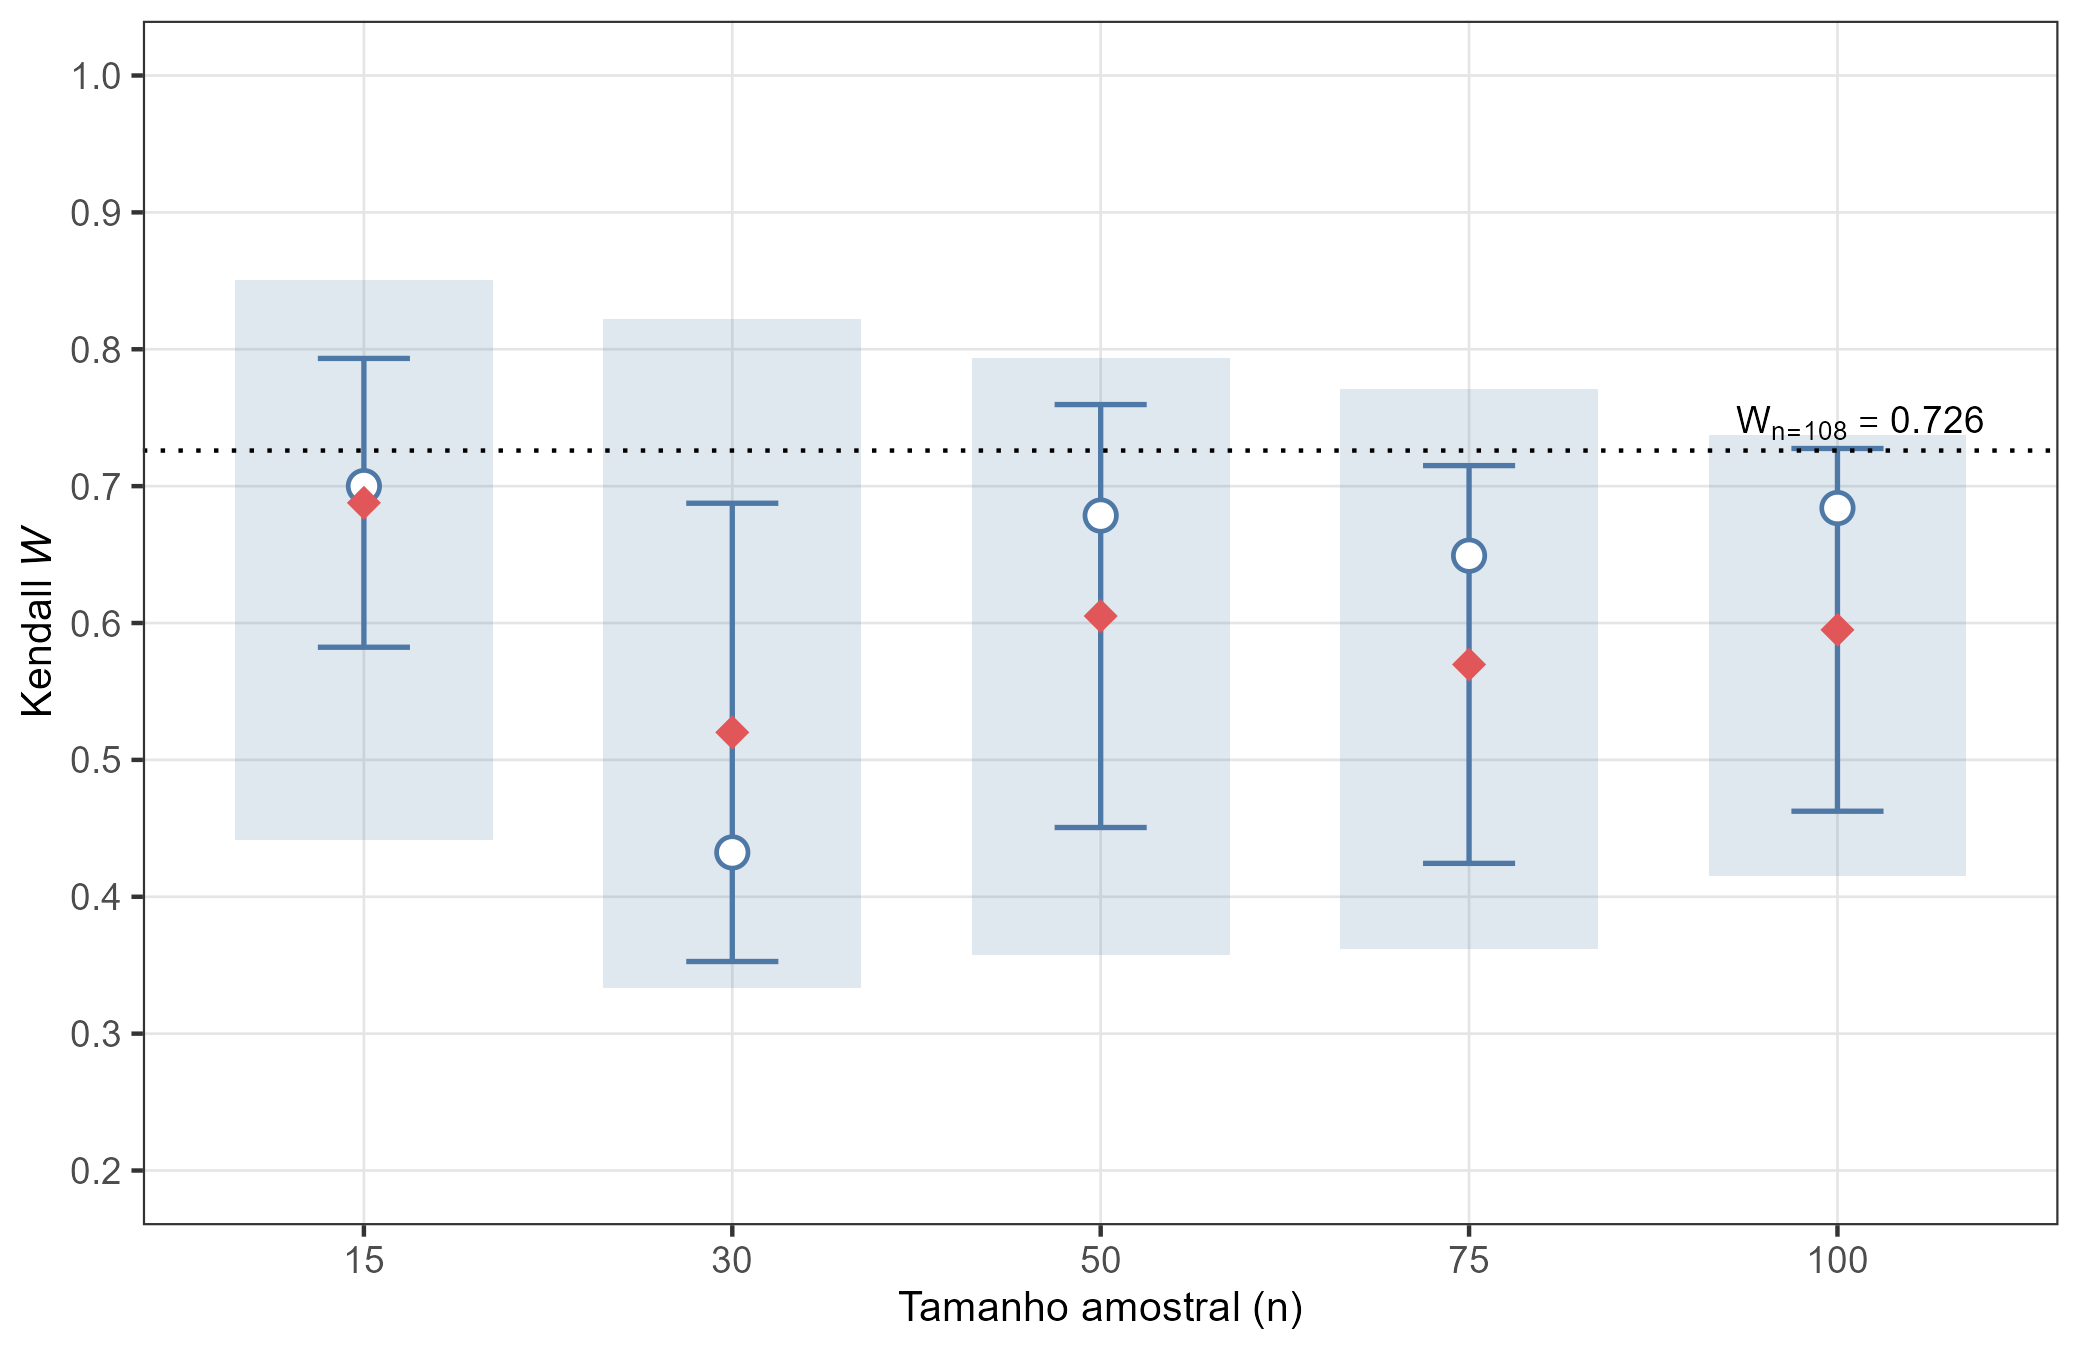
\includegraphics[width=0.75\textwidth]{../../2-DADOS/3-FIGURAS/fig_mc_sensitivity_34.png}
\caption{Distribuição do coeficiente de Kendall ($W$) em função do tamanho amostral ($n$), obtida por 200 iterações Monte Carlo estratificadas por célula do delineamento fatorial.}\label{fig:mc_box}
\smallskip\noindent\textit{Nota:} Losangos vermelhos indicam a média ($\bar{W}$); círculos brancos, a mediana; barras verticais, $\bar{W} \pm s$; retângulos sombreados, intervalo de percentis 2,5--97,5\%; linha pontilhada indica $W$ da amostra completa ($n = 108$).
\end{figure}

Diferentemente do cenário com 18 indicadores, não se observou estabilização de $\bar{W}$ a partir de $n = 30$. A reta GLS ajustada sobre $\log(n)$ indicou tendência negativa ($\hat{\beta}_1 = -0{,}037$), sem significância estatística ($p = 0{,}445$, $R^2 = 0{,}204$), refletindo a ausência de relação monotônica entre tamanho amostral e concordância. Esse padrão pode decorrer da maior dimensionalidade do vetor de indicadores ($q = 34$), que amplia a instabilidade do PLS-SEM em subamostragens (razão $n/q$ inferior a 2 em $n = 50$) e torna o proxy baseado em média aritmética insufficiente para reproduzir a estrutura de pesos do modelo completo. A dispersão dos percentis 2,5--97,5\% manteve-se elevada em todos os tamanhos amostrais (amplitude interquartílica $> 0{,}30$), indicando que a incerteza algorítmica não foi atenuada pelo aumento de $n$.

A instabilidade de $\bar{W}$ pode refletir tanto o número reduzido de níveis amostrais ($k = 5$), que limita a potência estatística do teste \citep{Mundform2005}, quanto a inadequação do proxy de PLS-SEM na subamostragem, que injeta variância espúria na concordância pentaparadigmática. \cite{Adak2023}, ao aplicarem IQS sob manejos contrastantes de preparo, resíduo e nitrogênio em rotação milho--trigo na planície Indo-Gangética, verificaram que amostras com $n < 30$ inflaram a incerteza dos pesos derivados de ACP, desestabilizando o ranqueamento dos tratamentos e produzindo inversões de posição entre manejos que, com a amostra completa ($n = 96$), eram estatisticamente distintos.

Esse padrão indica que a subamostragem introduz variabilidade que se sobrepõe às diferenças reais entre paradigmas, e que a ampliação do vetor de indicadores para 34 variáveis pode ter intensificado essa instabilidade ao reduzir a razão $n/q$ efetiva. Exercícios de \textit{benchmarking} conduzidos com $n < 50$ e $q > 30$ operam, portanto, em faixa de elevada instabilidade ($\bar{W} < 0{,}69$, $s > 0{,}10$), na qual as conclusões sobre superioridade ou inferioridade de um paradigma são indistinguíveis do ruído amostral.

\subsection{Implicações para monitoramento e transferibilidade}\label{subsec:implications}

Quando o interesse recai sobre ranqueamento de combinações manejo--cobertura em bases com $n \geq 50$, qualquer representante do bloco não linear (SIF, MARS ou RF) pode ser adotado com baixo risco de inversão ($\rho > 0{,}99$), possivelmente dispensando análise de sensibilidade ao paradigma.

Se a interpretabilidade dos caminhos causais entre domínios edáficos for prioritária, conforme recomendado em avaliações de indicadores compostos \citep{Cardoso2013}, o PLS-SEM oferece alternativa com incerteza moderada em relação ao bloco não linear (LoA\,$\approx \pm 1{,}58$), embora a exclusão de indicadores por multicolinearidade possa comprometer a representatividade do domínio físico. O paradigma ANOVA/MDS tende a divergir substancialmente do bloco não linear ($\rho \approx 0{,}28$; LoA\,$\approx \pm 2{,}40$), produzindo inversões em 67\% das combinações, e permanece indicado sobretudo para compatibilidade com o extenso acervo de estudos que adotaram o protocolo de \cite{Andrews2002} e para bases com número reduzido de indicadores ($q < 10$), condição na qual o ganho de precisão preditiva dos métodos não lineares tende a ser marginal \citep{Bünemann2018}. Esse protocolo de seleção, esquematizado na Fig.~\ref{fig:flowchart}, pode servir como referência para pesquisadores e extensionistas que necessitem justificar a escolha metodológica e quantificar a incerteza associada em avaliações de qualidade do solo.

\begin{figure}[!htb]
\centering
\resizebox{\textwidth}{!}{%
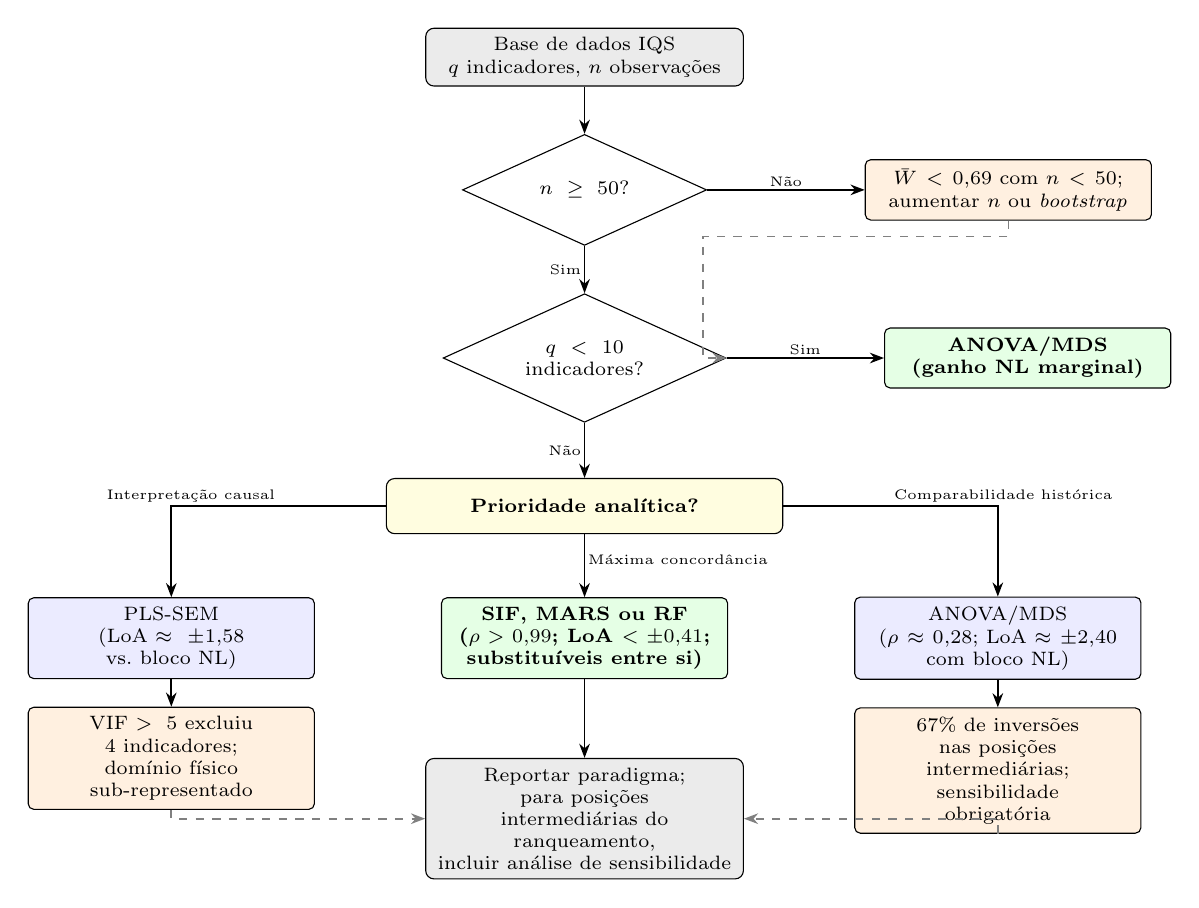
\begin{tikzpicture}[
    % --- node styles ---
    startend/.style={rectangle, rounded corners=3pt, minimum width=4cm,
        minimum height=0.6cm, text centered, draw=black, fill=black!8,
        font=\scriptsize, text width=3.8cm},
    dec/.style={diamond, aspect=2.2, minimum width=0.8cm,
        text centered, draw=black, fill=white,
        font=\scriptsize, text width=2.4cm, inner sep=1pt},
    prio/.style={rectangle, rounded corners=3pt, minimum width=5cm,
        minimum height=0.7cm, text centered, draw=black, fill=yellow!12,
        font=\scriptsize\bfseries, text width=4.8cm},
    rec/.style={rectangle, rounded corners=2pt, minimum width=3.6cm,
        minimum height=0.5cm, text centered, draw=black, fill=green!10,
        font=\scriptsize\bfseries, text width=3.4cm},
    proc/.style={rectangle, rounded corners=2pt, minimum width=3.6cm,
        minimum height=0.5cm, text centered, draw=black, fill=blue!8,
        font=\scriptsize, text width=3.4cm},
    warn/.style={rectangle, rounded corners=2pt, minimum width=3.6cm,
        minimum height=0.5cm, text centered, draw=black, fill=orange!12,
        font=\scriptsize, text width=3.4cm},
    % --- arrow / label styles ---
    arr/.style={-{Stealth[length=1.8mm]}, semithick},
    lbl/.style={font=\tiny, fill=white, inner sep=1pt},
    node distance=0.55cm and 1.6cm
]

%%% ================= ROW 0: ENTRADA =================
\node (start) [startend]
    {Base de dados IQS\\$q$ indicadores, $n$ observa\c{c}\~{o}es};

%%% ================= ROW 1: GATE amostral =================
\node (d1) [dec, below=0.6cm of start] {$n \geq 50$?};
\node (w1) [warn, right=2cm of d1]
    {$\bar{W} < 0{,}69$ com $n < 50$;\\aumentar $n$ ou \textit{bootstrap}};

%%% ================= ROW 2: GATE dimensionalidade =================
\node (d2) [dec, below=0.6cm of d1] {$q < 10$\\indicadores?};
\node (r_lowq) [rec, right=2cm of d2]
    {ANOVA/MDS\\(ganho NL marginal)};

%%% ================= ROW 3: RAMIFICA\c{C}\~{A}O POR PRIORIDADE =================
\node (prio) [prio, below=0.7cm of d2]
    {Prioridade anal\'{i}tica?};

%%% ================= ROW 4: TR\^{E}S RECOMENDA\c{C}\~{O}ES =================
\node (nlrec) [rec, below=0.8cm of prio]
    {SIF, MARS ou RF\\($\rho > 0{,}99$; LoA $< \pm 0{,}41$;\\substitu\'{i}veis entre si)};
\node (pls)   [proc, left=1.6cm of nlrec]
    {PLS-SEM\\(LoA $\approx \pm 1{,}58$\\vs.\ bloco NL)};
\node (anova) [proc, right=1.6cm of nlrec]
    {ANOVA/MDS\\($\rho \approx 0{,}28$; LoA $\approx \pm 2{,}40$\\com bloco NL)};

%%% ================= ROW 5: RESSALVAS =================
\node (pls_w)   [warn, below=0.35cm of pls]
    {VIF $> 5$ excluiu 4 indicadores;\\dom\'{i}nio f\'{i}sico sub-representado};
\node (anova_w) [warn, below=0.35cm of anova]
    {67\% de invers\~{o}es nas posi\c{c}\~{o}es\\intermedi\'{a}rias; sensibilidade\\obrigat\'{o}ria};

%%% ================= ROW 6: SA\'{I}DA =================
\node (endnode) [startend, below=1cm of nlrec]
    {Reportar paradigma; para posi\c{c}\~{o}es\\intermedi\'{a}rias do ranqueamento,\\incluir an\'{a}lise de sensibilidade};

%%% ================= SETAS =================
%% Gates bin\'{a}rios
\draw [arr] (start) -- (d1);
\draw [arr] (d1) -- node[lbl, left] {Sim} (d2);
\draw [arr] (d1) -- node[lbl, above] {N\~{a}o} (w1);
\draw [arr] (d2) -- node[lbl, left] {N\~{a}o} (prio);
\draw [arr] (d2) -- node[lbl, above] {Sim} (r_lowq);

%% Ramifica\c{c}\~{a}o tripla a partir de PRIORIDADE
\draw [arr] (prio.south) -- node[lbl, right, pos=0.4]
    {M\'{a}xima concord\^{a}ncia} (nlrec);
\draw [arr] (prio.west) -| node[lbl, above left, pos=0.25]
    {Interpreta\c{c}\~{a}o causal} (pls);
\draw [arr] (prio.east) -| node[lbl, above right, pos=0.25]
    {Comparabilidade hist\'{o}rica} (anova);

%% Ressalvas
\draw [arr] (pls) -- (pls_w);
\draw [arr] (anova) -- (anova_w);

%% Converg\^{e}ncia para sa\'{i}da
\draw [arr] (nlrec) -- (endnode);
\draw [arr, dashed, gray] (pls_w.south) |- (endnode.west);
\draw [arr, dashed, gray] (anova_w.south) |- (endnode.east);

%% Retorno: $n < 50$
\draw [arr, dashed, gray] (w1.south) |- ([yshift=-0.2cm]w1.south) -| ([xshift=1.5cm]d1.south) |- (d2.east);

\end{tikzpicture}%
}% end resizebox
\caption{Fluxograma decis\'{o}rio para sele\c{c}\~{a}o de paradigma de IQS.}\label{fig:flowchart}
\smallskip\noindent\textit{Nota:} Caixas verdes, recomenda\c{c}\~{a}o prim\'{a}ria; azuis, alternativa com ressalva; laranjas, advert\^{e}ncia operacional; amarela, n\'{o} de ramifica\c{c}\~{a}o multicrit\'{e}rio. Limiares de $\rho$ e LoA derivados da Tabela~\ref{tab:blandaltman}; invers\~{o}es de posto documentadas na Tabela~\ref{tab:ranking}.
\end{figure}

A generalização destes achados requer cautela. Os dados provêm de experimento conduzido sobre Argissolo com camada coesa \citep{LimaNeto2010} sob clima As$'$, condição na qual relações não lineares entre indicadores podem ser acentuadas pelo impedimento físico subsuperficial. Solos sem restrição física, ou sistemas com menor diversidade de práticas, poderiam exibir concordância inter-paradigma mais elevada, reduzindo a diferenciação entre famílias analíticas. \cite{Zhao2022}, em solo negro submetido a 19 anos de manejo conservacionista na China, verificaram que atributos físicos (estabilidade de agregados, porosidade) foram mais sensíveis ao tipo de preparo do que indicadores químicos, os quais responderam predominantemente à adubação. 

Em solos tropicais com camada coesa, a contribuição dos atributos físicos para o IQS tende a ser comprimida pela baixa diferenciação espacial na profundidade amostrada, o que pode amplificar a divergência entre paradigmas que competem por variância explicável em poucos indicadores físicos.

Comparações com Ultisols do Sudeste Asiático reforçam a aplicabilidade regional dos achados: \cite{Pheap2025}, em experimento de rotação arroz--leguminosa no Camboja, verificaram que a inferência fuzzy detectou benefícios de manejo conservacionista que o IQS aditivo não distinguiu, com concordância entre paradigmas não lineares ($\rho > 0{,}96$) semelhante à observada neste estudo. \cite{Briliawan2022}, em sistema agroflorestal sobre Ultisol da Indonésia, reportaram convergência entre RF e SIF (LoA\,$\approx \pm 0{,}51$), corroborando que a substituibilidade do bloco não linear pode ser generalizada para solos tropicais de baixa fertilidade intrínseca. A aplicação deste mesmo \textit{framework} a bases provenientes de outras classes de solo, particularmente Latossolos argilosos do Cerrado, onde \cite{DosSantos2021} já indicaram a eficácia do IQS fuzzy na diferenciação entre sistemas de cobertura, constitui direção promissora para consolidar os limiares de concordância aqui propostos.


%% ================================================================
%%                    SEÇÃO 5: CONCLUSÃO
%% ================================================================
\section{Conclusão}\label{sec:conclusion}

Os cinco paradigmas convergiram na identificação dos manejos extremos, porém 67\% das combinações intermediárias alteraram de posição conforme a família analítica, indicando que a escolha do método de agregação pode condicionar recomendações conservacionistas. Paradigmas não lineares (SIF, MARS, RF) mostraram-se praticamente intercambiáveis entre si ($\rho > 0{,}99$, LoA\,$< \pm 0{,}41$), ao passo que a ANOVA/MDS divergiu substancialmente do bloco não linear ($\rho \approx 0{,}28$), com inversões de até 8 posições no ranqueamento. A inclusão de indicadores dos domínios microbiológico, agronômico e de rendimento ampliou a divergência entre famílias lineares e não lineares (Wilcoxon $W = 18$, $p = 0{,}012$), sugerindo que vetores multidimensionais de indicadores tendem a acentuar, e não a atenuar, a sensibilidade do IQS à escolha do paradigma analítico. O cultivo mínimo com leguminosas (guandu) parece constituir a combinação mais consistente entre as abordagens testadas (Borda\,=\,92,6). Avaliações de IQS destinadas a subsidiar políticas de conservação podem beneficiar-se da inclusão de pelo menos um paradigma não linear e de análise de sensibilidade inter-paradigma para posições intermediárias do ranqueamento.

\backmatter


\bmhead{Agradecimentos}

Os autores agradecem aos técnicos do Campus Rural da Universidade Federal de Sergipe pelo suporte na condução do experimento de longa duração e na coleta de amostras de solo.

\section*{Declarações}

\begin{itemize}
\item \textbf{Financiamento:} 

O presente trabalho foi realizado com apoio da Coordenação de Aperfeiçoamento de Pessoal de Nível Superior -- Brasil (CAPES) -- Código de Financiamento 001 e do Conselho Nacional de Desenvolvimento Científico e Tecnológico (CNPq).
\item \textbf{Conflito de interesses:} 

Os autores declaram não possuir interesses concorrentes.
\item \textbf{Aprovação ética:} 

Não aplicável.
\item \textbf{Consentimento para publicação:} 

Não aplicável.
\item \textbf{Disponibilidade de dados e código:} 

O conjunto de dados anonimizado e todas as rotinas de análise (R e Python) utilizadas neste estudo encontram-se disponíveis em [URL DO REPOSITÓRIO]. As Tabelas Suplementares S1--S4 apresentam a saída completa da ANOVA, a base de regras fuzzy, os coeficientes de caminho do PLS-SEM e os ranqueamentos de importância de variáveis.
\item \textbf{Contribuição dos autores:} 

\textbf{A. Pedrotti}: Supervisão, Administração do projeto, Recursos, Investigação, Obtenção de financiamento. \textbf{L.D.V. Santos}: Conceitualização, Metodologia, Software, Análise formal, Visualização, Redação -- versão original. \textbf{J.A. Santos}: Investigação, Curadoria de dados. \textbf{S.J.A. Santos}: Investigação, Curadoria de dados. \textbf{J.S. Araújo}: Investigação, Curadoria de dados. \textbf{R.N. Araújo Filho}: Metodologia, Validação, Redação -- revisão e edição. \textbf{E.G. Silva}: Investigação, Curadoria de dados. \textbf{B.M.S. Andrade}: Investigação, Curadoria de dados. \textbf{F.S.R. Holanda}: Supervisão, Recursos, Obtenção de financiamento. Todos os autores leram e aprovaram a versão final do manuscrito.
\end{itemize}

\begin{appendices}

\section{Base de regras fuzzy completa}\label{secA2}

%% [A INSERIR]

\section{Coeficientes de caminho PLS-SEM e diagnósticos}\label{secA3}

%% [A INSERIR]

\end{appendices}

\bibliography{sn-bibliography}% common bib file

\end{document}
